\documentclass[journal]{IEEEtran}
\IEEEoverridecommandlockouts

\usepackage{cite}
\usepackage{amsmath,amssymb,amsfonts}
\usepackage{algorithmic}
\usepackage{graphicx}
\usepackage{textcomp}
\usepackage{xcolor}
\usepackage{hyperref}
\usepackage{float}
\usepackage{multirow}
\usepackage{booktabs}
\usepackage{colortbl}

% ── Palette for the unified results table (AUC heatmap + collapse shading) ──
\definecolor{aucPerfect}{HTML}{3DBC6E} % AUC ~1.00  strong green
\definecolor{aucStrong}{HTML}{8FCB7F}  % AUC ~0.95  green
\definecolor{aucMid}{HTML}{D7DC79}     % AUC ~0.84  lime
\definecolor{aucWeak}{HTML}{F0A85C}    % AUC ~0.59  orange
\definecolor{aucBad}{HTML}{E8736A}     % AUC ~0.57  red
\definecolor{collapseRed}{HTML}{F7D4D7}% collapsed binary config
\definecolor{funcGreen}{HTML}{D6EFD9}  % strongest binary config
\definecolor{grpBin}{HTML}{FBEFD9}     % "Binary" group header tint
\definecolor{grpScore}{HTML}{E2ECFB}   % "Similarity" group header tint

\newcommand{\note}[1]{\textcolor{red}{[#1]}}
% Placeholder for RidgeBase numbers still being computed (v2). Every \ph{...}
% renders in bold red so unfilled results are impossible to miss; grep '\\ph{'
% to find all remaining gaps before submission.
\newcommand{\ph}[1]{{\color{red}\textbf{[#1]}}}

\graphicspath{{figures/}}

\def\BibTeX{{\rm B\kern-.05em{\sc i\kern-.025em b}\kern-.08em
    T\kern-.1667em\lower.7ex\hbox{E}\kern-.125emX}}

\begin{document}

% ────────────────────────────────────────────────────────────────────────────
\title{SLAPBench: Benchmarking Multimodal Large Language Models\\
       for Four-Finger SLAP Fingerprint Verification}

% ─────────────────────────────────────────────────────────────────────────────
% DOUBLE-BLIND SUBMISSION (ECCV 2026 FoundGen-Bio workshop).
% Author block is anonymized for review. Restore the version below for the
% camera-ready:
%
%   \author{%
%     \IEEEauthorblockN{Bibesh Pyakurel and M.~G.~Sarwar Murshed}
%     \IEEEauthorblockA{\textit{Computer Science Department} \\
%     \textit{University of Wisconsin - Green Bay, Green Bay, WI, USA}}
%   }
% ─────────────────────────────────────────────────────────────────────────────
\author{%
  \IEEEauthorblockN{Anonymous FoundGen-Bio submission}
  \IEEEauthorblockA{Paper ID \note{XXXX}}
}

\maketitle

% ────────────────────────────────────────────────────────────────────────────
\begin{abstract}
Four-finger SLAP (Slap Livescan Acquisition Protocol) fingerprint images
are the standard capture format at every US border entry
point~\cite{nist_sd302}, yet no benchmark exists to determine whether
multimodal large language models (MLLMs) can verify identity from them.
%
We introduce \textbf{SLAPBench}, the first benchmark for MLLM evaluation
on four-finger SLAP fingerprint verification, built on NIST Special
Database 302b (SD302b), an operational nail-to-nail dataset of 201
participants captured at 500 and 1000~PPI across multiple devices.
%
We construct 7,832 verification pairs under an impostor-heavy all-pairs
protocol (176~mated, 7,656~non-mated) and evaluate four open-source
models (InternVL3-8B-Instruct, Qwen2.5-VL-7B-Instruct,
Qwen3-VL-8B-Instruct, and Gemma-3-12B-IT) together with the proprietary
Claude Opus~4.8 under three prompting strategies: zero-shot, task
description, and a continuous similarity-scoring prompt.
%
Task-description prompting collapses all four open-source models to
near-100\% False Accept Rate~(FAR), and Gemma-3-12B collapses under
zero-shot as well. Claude Opus~4.8 alone resists collapse under both
prompts and attains the strongest binary result (FAR~$= 20.2\%$).
%
The similarity-scoring prompt eliminates collapse across the open-source
models and separates them into a clear ranking. We verified directly, however,
that on SD302b a mated pair is the 500 and 1000~PPI versions of a
\emph{single} capture---the 500~PPI image is an exact 2$\times$ downscale
(mean pixel difference $<1/255$)---so this ranking indexes
\emph{near-duplicate sensitivity}, not verification capability, and we report
it as such: Claude Opus~4.8 reaches Area Under the ROC Curve (AUC)~$= 0.953$
and Gemma-3-12B~$= 0.837$, whereas InternVL3-8B and Qwen2.5-VL-7B are near
random ($0.590$ and $0.567$), and Qwen3-VL-8B separates the classes perfectly
(AUC~$= 1.000$)---perfect \emph{near-duplicate detection} rather than
fingerprint matching. Because SD302b supplies only one SLAP capture per finger
position, no genuine same-finger, independent-impression pair can be formed
from it at all. We therefore read these SD302b genuine-pair scores as a
cautionary finding about how MLLM biometric benchmarks are assembled, and we
address it directly rather than only caveat it.
%
To measure genuine verification, we extend the benchmark to \textbf{RidgeBase}, a
cross-sensor contactless four-finger dataset that provides multiple
\emph{independent} captures per hand, and add a prompt-free embedding-matching
evaluation alongside prompting. On these independent-capture pairs the perfect
SD302b separation does not replicate: every open-source model falls to chance
(embedding AUC~$0.40$--$0.51$, similarity-scoring AUC~$0.50$--$0.56$), none can
tell a subject's own two hands apart (same-person different-hand diagnostic
AUC~$0.52$--$0.58$), and the task-description collapse recurs (FAR~$98$--$100\%$).
What little residual signal exists is sensor consistency, not identity: the
strongest model's genuine-pair AUC drops from $0.64$ within a device to $0.49$
across devices. Current MLLMs thus match global appearance rather than ridge
structure on four-finger images.
%
A stratified analysis across gender, race, and age finds that demographic
disparity tracks model \emph{weakness} rather than strength, inverting the
pattern reported for face benchmarks, though small subgroup sizes make
this an initial probe rather than a definitive audit.
Together these results establish the first SLAP-specific MLLM
verification baseline and show that prompt format governs whether collapse
occurs, that near-perfect scores on a single-capture benchmark can be an
artifact of pair construction, and that on genuinely independent captures no
current MLLM verifies four-finger fingerprints.
\end{abstract}

\begin{IEEEkeywords}
fingerprint verification, SLAP fingerprint, multimodal large language
models, biometric benchmark, NIST SD302b, zero-shot evaluation,
similarity scoring, positive-bias collapse, InternVL3, Qwen2.5-VL, Qwen3-VL, Gemma~3, Claude Opus
\end{IEEEkeywords}

% ────────────────────────────────────────────────────────────────────────────
\section{Introduction}
\label{sec:intro}

Every US border entry point verifies traveler identity through a
\emph{SLAP} (Slap Livescan Acquisition Protocol) impression: four
fingers pressed simultaneously against a flat-bed scanner, matched
against the IDENT (DHS Automated Biometric Identification System)
database~\cite{nist_sd302}.
Unlike the rolled or plain single-finger impressions used in all prior
fingerprint MLLM benchmarks~\cite{fpbench2025}, SLAP images place four
overlapping fingers in a single frame, introduce ridge quality variation
across the capture, and require spatial reasoning about inter-finger
relationships.
SD302b sharpens the challenge further: collected at enrollment speed
during live border deployment, it is operational data, not a
competition set designed for controlled algorithmic evaluation.

Despite this operational importance, SLAP fingerprint images have not
been evaluated in any multimodal LLM benchmark.
The closest prior work, FPBench~\cite{fpbench2025}, evaluates 20~MLLMs on
eight fingerprint tasks, but every task uses \emph{individual} rolled or
plain impressions drawn from Fingerprint Verification Competition (FVC)
datasets and NIST SD302d/SD301a, collected from a single isolated finger
under controlled laboratory conditions.
No prior fingerprint MLLM benchmark exercises the inter-finger spatial
reasoning that SLAP images require.

A second open question concerns how prompting strategy affects collapse.
Benchmarks across face and fingerprint biometrics have documented
\emph{positive-bias collapse}, in which a model selects the same answer
(``same person'') regardless of input and thereby achieves exactly 50\%
accuracy on a balanced test set while appearing to
function~\cite{facerecbench2025,fpbench2025}.
Binary forced choice is the format used in every prior biometric MLLM
benchmark. Whether it induces the same collapse on SLAP data, and whether
alternative prompt designs can prevent it, bears directly on a failure
mode that no border security application could tolerate: a system that
accepts every traveler as genuine.
We stress that SLAPBench is an \emph{evaluation probe} of current MLLM
behavior on SLAP-format images, not a proposed deployment system. Our aim
is to characterize how these models succeed and fail under different
prompts, not to advocate their use in operational border verification.

This paper makes the following contributions:

\begin{enumerate}
  \item \textbf{SLAPBench}, the first benchmark for MLLM evaluation on
        four-finger SLAP fingerprint verification, built on NIST SD302b, an
        operational dataset that no prior fingerprint MLLM work has used.

  \item \textbf{A reproducible evaluation protocol} of 7,832~fixed pairs
        (176~mated, formed across resolution because SD302b provides a
        single SLAP capture per finger position; 7,656~non-mated, covering
        all $\binom{88}{2}$ subject combinations per FRGP), released as a
        fixed pair manifest with demographic metadata that supports a
        stratified analysis across gender, race, and age.

  \item \textbf{Systematic evidence of positive-bias collapse on SLAP data.}
        Five of ten binary prompting configurations collapse to accepting
        nearly every pair as genuine. All four open-source models collapse
        under task-description prompting and Gemma-3-12B collapses under
        zero-shot as well, while the proprietary Claude Opus~4.8 resists
        collapse under both prompts. Collapse is therefore largely a
        property of the prompt format, but a sufficiently capable model can
        overcome it.

  \item \textbf{A similarity-scoring prompt that removes collapse.}
        Continuous scoring eliminates the constant-output collapse in all four
        open-source models, so it is necessary for any signal to appear. On
        SD302b the resulting score separation reflects near-duplicate
        sensitivity rather than verification (mated pairs are same-capture
        cross-resolution), and we treat it as such
        (Table~\ref{tab:main_results}); genuine verification is measured only on
        RidgeBase (contribution~6).

  \item \textbf{A resolved analysis of a perfect benchmark score.}
        Qwen3-VL-8B attains AUC~$= 1.000$ under scoring. We show that on SD302b,
        where every mated pair is a 500/1000~PPI rendering of one capture, this
        is near-duplicate detection rather than verification, and we confirm it
        empirically: on independent RidgeBase captures the same model falls to
        chance. Near-perfect MLLM biometric results warrant a protocol audit,
        or an independent-capture dataset, before they are read as capability.

  \item \textbf{An independent-capture cross-sensor evaluation on RidgeBase.}
        We extend the benchmark to RidgeBase~\cite{ridgebase2022}, whose
        multiple independent captures per hand remove the same-capture confound
        of SD302b, and add (i)~a prompt-free embedding-matching evaluation of
        each open-source model's vision encoder, (ii)~a controlled
        same-device/cross-device split, and (iii)~a same-person/different-hand
        diagnostic that isolates appearance matching from ridge matching. Every
        model sits at chance on genuine verification here, establishing that the
        SD302b perfect score does not reflect fingerprint-matching ability
        (Section~\ref{sec:rb_results}).

  \item \textbf{Public release} of the evaluation code, the fixed pair
        manifest, the raw result CSVs, and the per-pair score files, so that
        every number reported here can be recomputed. The repository link is
        withheld for double-blind review and will be included in the
        camera-ready version.
\end{enumerate}

The remainder of this paper is organized as follows.
Section~\ref{sec:related} reviews related work in fingerprint recognition,
MLLM benchmarking, and biometric LLM evaluation.
Section~\ref{sec:dataset} describes the NIST SD302b dataset and our
data preparation pipeline.
Section~\ref{sec:method} defines the evaluation protocol, pair construction
methodology, and prompting strategies.
Section~\ref{sec:results} presents experimental results and analysis.
Section~\ref{sec:discussion} discusses implications and limitations.
Section~\ref{sec:conclusion} concludes.

% ────────────────────────────────────────────────────────────────────────────
\section{Related Work}
\label{sec:related}

\subsection{Fingerprint Recognition}

Traditional fingerprint recognition systems operate on a well-defined
pipeline: image acquisition, enhancement, feature extraction (minutiae
or texture-based), and matching~\cite{maltoni_handbook}.
Deep learning has substantially advanced each stage: FingerNet unifies
ridge orientation and minutiae extraction in a CNN framework~\cite{fingerNet};
DeepPrint learns compact fixed-length embeddings for scalable
verification~\cite{deepprint}; transformer-based architectures combine
global and local representations with attention-based matching.
Commercial matchers such as VeriFinger~\cite{verifinger} establish
operational baselines with well-characterized False Accept Rate~(FAR)
and False Reject Rate~(FRR) operating curves.
These systems treat fingerprint recognition as a visual similarity
problem to be solved by dedicated learned representations, an approach
fundamentally different from the zero-shot visual reasoning that MLLMs
perform.

SLAP segmentation, the upstream step of extracting individual finger
regions from a four-finger image, has been studied in dedicated
work~\cite{murshed2024SlapSeg}, which provides segmentation ground truth
used in our dataset construction.
To our knowledge, no prior work has evaluated end-to-end MLLM performance
on SLAP-format images.

\subsection{MLLM Benchmarks for Biometrics}

Recent years have seen a proliferation of benchmarks probing MLLM
capabilities in domain-specific visual tasks.
FaceXBench~\cite{facexbench2024} evaluates 28~models on 5,000
multiple-choice questions covering 14 face-understanding tasks, finding
that the best MLLM (Qwen2-VL-72B at 57.86\%) trails human performance
(70.28\%) and specialized models (84.50\%) by substantial margins.
A key finding directly relevant to our work: chain-of-thought
(CoT) prompting consistently \emph{degraded} performance on face tasks,
cautioning against assuming CoT is universally beneficial.

FaceRecBench~\cite{facerecbench2025} benchmarks 27~MLLMs on six face
recognition datasets using the same protocol as classical face recognition
systems, making scores directly comparable to the non-LLM literature.
Qwen2-VL-7B achieved the best MLLM score at 81.10\%, against 97.31\% for
IResNet-50.
Critically, FaceRecBench documents that many MLLMs collapse to 50\% accuracy
on balanced test sets by always accepting or always rejecting pairs, and
that the best-performing model exhibits the strongest demographic bias.
Our work revisits both findings in the fingerprint domain.
The same research group extended this evaluation to heterogeneous face
recognition~\cite{shahreza2026hfr}, benchmarking MLLMs across cross-spectral
scenarios (VIS--NIR, VIS--SWIR, VIS--THERMAL) and reporting substantial
performance gaps between MLLMs and dedicated face recognition models. Those
gaps are consistent with what we observe on SLAP fingerprint images.

FPBench~\cite{fpbench2025} is the most directly relevant prior work.
It evaluates 20~MLLMs on eight fingerprint tasks across seven datasets.
Gemini 2.5 Pro leads at 57.01\% overall accuracy; GPT-5 follows at 50.20\%;
open-source models including InternVL3-38B (52.86\%) and Qwen3-VL-8B
(49.42\%) achieve competitive results.
Fine-tuning vision and language encoders jointly improves performance by
approximately 7--39\%~\cite{fpbench2025}.
FPBench's fingerprint verification task uses individual-finger images and
MCQ-format prompting.
Our work differs in three critical ways: (i)~we use four-finger SLAP images,
requiring spatial multi-finger reasoning; (ii)~we evaluate continuous
similarity scoring in addition to binary classification; and
(iii)~we use SD302b, an operational high-resolution dataset not used in
FPBench.

\subsection{Response Collapse in Binary Verification}

A recurring observation across biometric MLLM benchmarks is the tendency
of models to collapse toward a single response class in binary
verification tasks~\cite{facerecbench2025,fpbench2025}.
FaceRecBench documents models that achieve exactly 50\% accuracy on
balanced test sets by always predicting ``same person.''
FPBench reports similar degenerate behavior on fingerprint verification.
This collapse has been hypothesized to reflect training-data priors that
favor ``same'' responses, compounded by the ambiguity of biometric
comparison when expressed in natural language~\cite{facerecbench2025,fpbench2025}.
Our work provides the first quantitative documentation of this phenomenon
specifically on SLAP fingerprint images and demonstrates that continuous
scoring prompts can eliminate collapse and expose whatever discriminative
signal is present in the underlying model.

% ────────────────────────────────────────────────────────────────────────────
\section{Dataset and Data Preparation}
\label{sec:dataset}

\subsection{NIST Special Database 302b}

NIST SD302b~\cite{nist_sd302} is a subset of the Nail-to-Nail (N2N)
Fingerprint Challenge dataset collected by the Intelligence Advanced
Research Projects Activity (IARPA).
The database contains fingerprint images from 201~participants captured
using multiple devices at two resolutions: 500~PPI (standard operational
resolution) and 1000~PPI (high resolution for research).
Participants span diverse demographics including age (range: 18--70),
gender, race, and occupational background (work type), enabling
stratified fairness analysis.
We focus exclusively on \textbf{FRGP 13} (right four-finger SLAP) and
\textbf{FRGP 14} (left four-finger SLAP) images captured by
\textbf{Device~R}.
Device~R images in SD302b are captured natively at 1000~PPI, and the
corresponding 500~PPI versions are supplied for compatibility with
500~PPI fingerprint algorithms. The 500~PPI image is therefore a
downsampled version of the same capture rather than a second, independent
impression.
We confirmed this directly against the distributed file structure rather
than relying on the documentation alone. Across the 88~clean subjects, the
Device~R SLAP set contains exactly 352~files, one per
(subject,~FRGP,~resolution) triple, and every file name has the form
\texttt{SUBJECT\_R\_\{500\textbar1000\}\_slap\_\{13\textbar14\}.png} with
no impression or sequence index. Each (subject,~FRGP) combination is
therefore represented by exactly one capture, available at two resolutions,
and SD302b offers no repeat SLAP impression for any subject and finger
position.
This is a property of the database rather than a choice on our part, and it
fixes the form a mated pair can take: each mated pair is a
\emph{same-capture cross-resolution} comparison between the native
1000~PPI image and its 500~PPI counterpart, not a comparison of two
independent impressions.
Sections~\ref{sec:pairs} and~\ref{sec:discussion} set out what this
structure does and does not permit us to conclude.

\subsection{Data Preparation}

Following the SD302b documentation, we apply three exclusion criteria:
(i)~\emph{errata} subjects flagged for documented labeling errors
(7~subjects, listed in the NIST errata log) are excluded from all pairs;
(ii)~roll images (devices U and V), FRGP~15 thumb-slap images, and
pre-cropped slap-segmented individual finger images are archived and
excluded from the benchmark;
(iii)~only subjects with matched pairs in both R-500 and R-1000 sets
are eligible for genuine pair construction.

The subject count reduces as follows: of the \textbf{201} participants in
SD302b, \textbf{92} have Device~R four-finger SLAP captures for both
FRGP~13 and~14 at both the native 1000~PPI and resampled 500~PPI
resolutions; removing errata-flagged and incomplete-record subjects leaves
\textbf{88} clean subjects (four subjects dropped, including
00002302 and 00002420, whose SD302b errata note swapped-finger labels).
The verification experiment therefore draws on \textbf{352 Device~R SLAP
images} (88~subjects $\times$ 2~FRGP positions $\times$ 2~resolutions).
These are a subset of a broader curated active set of \textbf{584 SLAP
images}, which additionally retains Device~S 500~PPI captures and the
excluded subjects' images for future SLAP tasks; only the 352 Device~R
images above enter the pair construction of this paper.
For each image, we build a master dataframe recording image-level
metadata (device, resolution, FRGP, dimensions, integrity checksum),
per-finger segmentation ground truth (bounding-box coordinates and
rotation angle $\theta$ from the SD302b segmentation CSVs), and
participant demographics.

\subsection{Ground-Truth Segmentation}
\label{sec:segmentation}

SD302b provides per-image segmentation CSVs listing bounding-box
coordinates (top-left, top-right, bottom-left, bottom-right corner
pixels) and a rotation angle $\theta$ for each of the four fingers.
These annotations, produced by the SLAP segmentation system
of~\cite{murshed2024SlapSeg}, enable future tasks including
localization evaluation and finger-level analysis.
Figure~\ref{fig:anatomy} shows a representative SLAP image with the four
finger regions overlaid from this ground truth.
For the verification task (the subject of this paper), we use the
full SLAP images without cropping, consistent with how these images
are consumed in operational border-entry pipelines.

\begin{figure}[t]
  \centering
  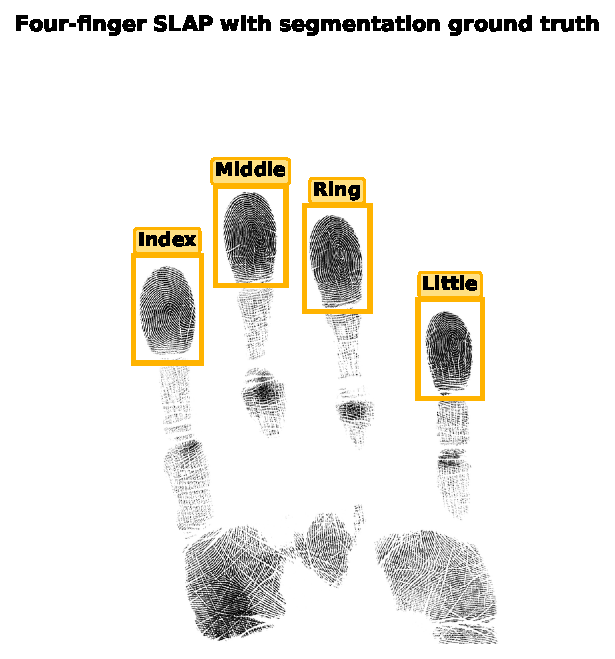
\includegraphics[width=0.74\columnwidth]{fig_slap_anatomy.pdf}
  \caption{A four-finger SLAP capture (NIST SD302b, Device~R, 500~PPI) with
    the per-finger segmentation ground truth overlaid (index, middle, ring,
    little). A single frame holds four overlapping fingers of broadly similar
    morphology. Any two SLAP images therefore look globally alike whether
    they are mated or not, which underlies the positive-bias collapse
    analyzed in Section~\ref{sec:discussion}.}
  \label{fig:anatomy}
\end{figure}

\subsection{RidgeBase: Independent-Capture Four-Finger Verification}
\label{sec:ridgebase}

The single-capture-per-position structure of SD302b (Section~\ref{sec:dataset})
fixes every mated pair as a same-capture cross-resolution comparison, which,
as Section~\ref{sec:discussion} details, admits a resolution shortcut and makes
a perfect score ambiguous. To resolve that ambiguity we add a second
evaluation on \textbf{RidgeBase}~\cite{ridgebase2022}, a cross-sensor
multi-finger contactless fingerprint dataset whose defining property is exactly
what SD302b lacks: \emph{multiple independent captures} of the same four-finger
hand. RidgeBase acquires each hand several times with different smartphones
(Apple and Google devices) across sessions, so a mated pair is a comparison of
two genuinely separate photographs rather than two resolutions of one image.

We use the four-finger contactless images of the RidgeBase Task~2 test split:
\textbf{25 subjects}, \textbf{50 (subject, hand) identities}, and \textbf{560
whole-hand images}, with every identity captured on both device families
($\geq$2 captures per hand). This is a contactless smartphone modality rather
than a contact livescan, and we treat it as a complementary stress test: it
holds the four-finger SLAP framing (four fingers of one hand imaged together)
while removing the same-capture confound and adding a genuine cross-sensor gap.
Because mated pairs are now independent captures, RidgeBase lets us separate two
explanations of the SD302b result---appearance matching versus ridge
matching---that SD302b alone cannot.

% ────────────────────────────────────────────────────────────────────────────
\section{Evaluation Protocol and Methodology}
\label{sec:method}

\subsection{Pair Construction}
\label{sec:pairs}

We construct mated and non-mated verification pairs following the
all-pairs protocol used in FaceRecBench~\cite{facerecbench2025} and
FPBench~\cite{fpbench2025}.

\textbf{Mated (genuine) pairs.}
For each FRGP $\in \{13, 14\}$, we pair each subject's native 1000~PPI
image with the corresponding downsampled 500~PPI version of the
\emph{same capture}.
With 88~clean subjects, this yields 88~mated pairs per FRGP and 176~mated
pairs in total.
Each eligible subject contributes exactly one such comparison per SLAP
position, so the count of mated comparisons is fixed at 176 by the
structure of the database rather than by a sampling decision.

\textbf{Non-mated (impostor) pairs.}
For each FRGP, we form all pairings of distinct subjects.
With 88 subjects, this yields $\binom{88}{2} = 3{,}828$ unique non-mated
pairs per FRGP, and $3{,}828 \times 2 = 7{,}656$ non-mated pairs in total.
We verify that no non-mated pair involves the same subject.
This exhaustive construction follows standard practice in biometric
benchmarking~\cite{facerecbench2025} and provides more reliable
error-rate estimates than random subsampling.

\textbf{An impostor-heavy, not balanced, protocol.}
The resulting set contains \textbf{7,832~pairs}
(176~mated $+$ 7,656~non-mated) and is released as a fixed pair manifest
to ensure identical evaluation across models.
This is an intentionally impostor-heavy all-pairs verification protocol,
not a balanced dataset: non-mated trials grow combinatorially with the
number of enrolled subjects while mated trials are limited by the
available samples per subject.
Such imbalance is standard in biometric evaluation, and we therefore
emphasize FAR, FRR, ROC-AUC, EER, and TAR at low FAR throughout, rather
than overall accuracy, which is dominated by the majority (non-mated)
class.

\textbf{Resolution structure and its consequence.}
Mated pairs are cross-resolution (1000~PPI vs.\ 500~PPI), whereas
non-mated pairs are drawn from the 500~PPI pool and are therefore
same-resolution (500~PPI vs.\ 500~PPI).
The two classes consequently differ in a property that has nothing to do
with identity, and a model could in principle separate them by reading
resolution or appearance statistics instead of comparing ridge structure.
We state this plainly at the outset because it governs how the strongest
results in Section~\ref{sec:results} may be read, and we return to it in
Section~\ref{sec:perfect}.
Accordingly, we do \emph{not} read the SD302b similarity-scoring separation as
a verification-capability ranking; it indexes near-duplicate sensitivity, and
genuine verification is measured instead on the independent-capture RidgeBase
data (Section~\ref{sec:rb_results}), which removes the asymmetry at its source
rather than controlling for it within SD302b.
The collapse results are not affected and carry no such caveat, for the
reason given in Section~\ref{sec:limitations}: FAR is computed on non-mated
pairs, which are same-resolution by construction and involve no
cross-resolution comparison at all.
Each pair record also carries demographic metadata (age, gender, and race
of both subjects), which supports the stratified analysis in
Section~\ref{sec:fairness}.

\subsection{RidgeBase Pair Construction and Embedding Evaluation}
\label{sec:rb_pairs}

On RidgeBase (Section~\ref{sec:ridgebase}) the identity unit is the
(subject, hand) pair, since a hand is a fixed set of four fingers. We build
three comparison categories:
\begin{itemize}
  \item \textbf{Genuine (mated):} same subject, same hand, two \emph{different}
        independent captures. Unlike SD302b, these are separate photographs,
        not two resolutions of one image.
  \item \textbf{Primary impostor (non-mated):} different subjects, same hand.
  \item \textbf{Diagnostic impostor (non-mated):} same subject, \emph{different}
        hand (left vs.\ right). These are the same person's two hands---identical
        skin tone, lighting, and background but genuinely different fingers---so
        they isolate whether a model keys on identity-level appearance cues
        rather than ridge structure.
\end{itemize}
Because every hand is captured on both device families, each genuine and each
primary-impostor pair is tagged \textbf{same-device} (Apple$\leftrightarrow$Apple
or Google$\leftrightarrow$Google) or \textbf{cross-device}
(Apple$\leftrightarrow$Google), giving a controlled cross-sensor split. We match
the impostor set's device composition to the genuine set so that any
genuine--impostor difference cannot be attributed to device makeup. The balanced
evaluation manifest contains \textbf{1{,}484 pairs} (592 genuine, 592 primary
impostor---each 277 same-device and 315 cross-device---and 300 diagnostic
impostors); a larger \textbf{4{,}461-pair} manifest is released for
higher-power analysis. As a construction check, the mean genuine similarity is
strictly below unity, confirming that mated pairs are independent captures and
not near-duplicates.

\textbf{Embedding-based verification.}
Beyond prompting, we add a prompt-free evaluation on RidgeBase that reads each
model's visual representation directly: we extract the image embedding from the
model's vision encoder, $\ell_2$-normalize it, and score a pair by cosine
similarity, then report AUC, EER, and TAR at FAR~$=0.1\%$ exactly as for the
similarity-scoring prompt. This measures whether the learned visual features
carry any identity signal independent of the language head, and is applied to
the four open-source models, whose vision towers are accessible; the
proprietary APIs do not expose image embeddings and are evaluated by prompting
only.

\subsection{Models}

We evaluate four open-source MLLMs and one proprietary frontier model,
selected for their demonstrated performance on fingerprint and face
biometric benchmarks and to span a range of model scales and access
modes (locally hosted open weights versus a commercial API):

\textbf{InternVL3-8B-Instruct}~\cite{internvl3} (OpenGVLab) is a
vision--language model built on an InternViT vision encoder and an
InternLM language model.
It was among the top open-source performers in FPBench~\cite{fpbench2025}.
We load it in bfloat16 precision, consuming approximately 16~GB VRAM.

\textbf{Qwen2.5-VL-7B-Instruct}~\cite{qwen25vl} (Alibaba) is the
architecture used in FaceRecBench~\cite{facerecbench2025}, where
Qwen2-VL-7B achieved 81.10\%, the highest MLLM result on that benchmark.
We load it with 4-bit NF4 quantization (bitsandbytes), consuming
approximately 6~GB VRAM.

\textbf{Qwen3-VL-8B-Instruct}~\cite{qwen3vl} (Alibaba) is the
successor to the Qwen2.5-VL series, featuring DeepStack multi-level
feature fusion, interleaved multi-resolution positional embeddings, and
a 256K native context window~\cite{qwen3vl}.
It is evaluated in FPBench~\cite{fpbench2025}, where it achieves 49.42\%
on single-finger tasks.
We load it with 4-bit NF4 quantization (bitsandbytes), consuming
approximately 6~GB VRAM.

\textbf{Gemma-3-12B-IT}~\cite{gemma3} (Google DeepMind) is a multimodal
model from the Gemma~3 family, pairing a SigLIP vision encoder with the
Gemma~3 language backbone. At 12~billion parameters it is the largest of
our four local models.
We load it with 4-bit NF4 quantization (bitsandbytes), consuming
approximately 8~GB VRAM.

\textbf{Claude Opus~4.8}~\cite{claudeopus} (Anthropic) is a proprietary
frontier MLLM included as a high-capability reference point against the
open-source models. We access it through the Anthropic API at its default
decoding settings; model weights, size, and architecture are not publicly
disclosed.

The four open-source models are loaded directly via the HuggingFace
\texttt{transformers} library without a serving layer on a single
NVIDIA RTX~4080~SUPER GPU (16.9~GB), ensuring deterministic inference
(\texttt{temperature}$=0$, \texttt{do\_sample=False}); Claude Opus~4.8 is
queried through the Anthropic API. To bound non-determinism in the API model, every Claude
pair is issued as a single independent request with no conversation
state, and the identical image preprocessing and prompt templates are
used across all five models.
The exact model identifiers evaluated are
\texttt{InternVL3-8B-Instruct}, \texttt{Qwen2.5-VL-7B-Instruct},
\texttt{Qwen3-VL-8B-Instruct}, \texttt{Gemma-3-12B-IT}, and the Anthropic
API model \texttt{claude-opus-4-8}.
All runs reported here were collected in June~2026.
The two images and the text prompt are the only inputs provided to each
model. No filenames, subject identifiers, resolution labels, or
demographic metadata appear in any request, so no model, local or API,
has access to ground-truth identity information at inference time.

\subsection{Prompting Strategies}
\label{sec:prompts}

We evaluate three prompting strategies, using a fixed system prompt
``\textit{You are an expert fingerprint examiner.}'' across all settings.
Before inference, every image is converted to grayscale, contrast-normalized
(autocontrast), and resized to $448\times448$ pixels, identically for all
five models; this common preprocessing also equalizes the pixel dimensions
of the 500 and 1000~PPI images, though it does not remove the underlying
near-duplicate relationship between a mated pair
(Section~\ref{sec:discussion}).
The three prompt templates are reproduced verbatim in
Figure~\ref{fig:prompts}.

\begin{figure*}[t]
\centering
\footnotesize
\setlength{\fboxsep}{6pt}
\noindent\fbox{\parbox{0.95\textwidth}{%
\textbf{System prompt (all strategies).}\\
{\ttfamily You are an expert fingerprint examiner.}

\vspace{4pt}\hrule\vspace{4pt}
\textbf{Zero-shot (ZS).}\\
{\ttfamily Below are two SLAP fingerprint images. A SLAP image captures four
fingers from one hand pressed simultaneously on a scanner.\\
Do these two images belong to the same person?\\
(A) Yes, same person\\
(B) No, different people\\
Reply with only the letter A or B.}

\vspace{4pt}\hrule\vspace{4pt}
\textbf{Task description (TD).}\\
{\ttfamily A SLAP fingerprint image captures four fingers from one hand
simultaneously. The same person's fingers produce slightly different images
each time they press the scanner (different pressure, slight movement), but
the ridge patterns remain the same.\\[2pt]
Below are two SLAP fingerprint images. Do these two images belong to the
same person?\\
(A) Yes, same person\\
(B) No, different people\\
Reply with only the letter A or B.}

\vspace{4pt}\hrule\vspace{4pt}
\textbf{Similarity scoring (SS).}\\
{\ttfamily You are a forensic fingerprint examiner analyzing two SLAP
fingerprint images. A SLAP image captures four fingers (index, middle, ring,
little) pressed simultaneously on a scanner.\\[2pt]
Your task: Examine the ridge flow patterns, ridge endings, bifurcations, and
the relative shape and spacing of each finger across both images. Then return
a single integer between 0 and 100 representing your confidence that both
images belong to the same person, where:\\
0 = 0\% confident (certain they are different people)\\
50 = 50\% confident (completely uncertain)\\
100 = 100\% confident (certain they are the same person)\\[2pt]
A score of 65 means you are 65\% confident the images are from the same
person. Reply with the number only. Do not include any text, explanation, or
label.}
}}
\caption{The three prompt templates, reproduced verbatim. Every model
  receives the same system prompt and, for each strategy, the same user
  prompt, with the two SLAP images attached to the user message. Here
  \texttt{\%} denotes a literal percent sign in the model input.}
\label{fig:prompts}
\end{figure*}

\textbf{Zero-shot (ZS).}
The model receives the two SLAP images and a minimal binary question:
\textit{``Do these two images belong to the same person?''} with
options (A) Yes and (B) No.
This is the standard protocol in FPBench and
FaceRecBench~\cite{fpbench2025,facerecbench2025}, enabling direct
comparison.

\textbf{Task description (TD).}
The prompt additionally explains the nature of SLAP images and the
effect of repeated captures (pressure variation, slight movement)
before posing the same binary question.
This tests whether domain context reduces the collapse tendency.

\textbf{Similarity scoring (SS).}
Rather than a binary choice, the model is asked to return a single
integer between 0 and 100 representing its confidence that the two
images belong to the same person: 0 means completely certain they are
different people; 100 means completely certain they are the same person.
The model is instructed to reply with the number only, with no
explanation or label.
This framing treats the model's output as a direct confidence
percentage, avoiding the need to cross a forced binary decision boundary.

\subsection{Response Parsing and Metrics}

For binary prompts (ZS, TD), we parse responses using a
three-step fallback strategy following VLMEvalKit~\cite{vlmevalkit}:
(1)~if the response starts with A or B, accept it;
(2)~if A or B appears anywhere in the response, accept it;
(3)~keyword matching on SAME/YES/GENUINE vs.\ DIFFERENT/NO/IMPOSTOR.
Responses matching none of these patterns are marked INVALID.

For the similarity scoring prompt, we extract the first integer in the
response via regex and clamp to $[0, 100]$. This tolerates the rare
case where a model prepends or appends text despite the instruction
to return a number only.

\textbf{Binary metrics} (ZS, TD):
overall accuracy, genuine accuracy (TAR), impostor accuracy (TNR),
FAR (impostor pairs incorrectly accepted), FRR (genuine pairs
incorrectly rejected), and collapse detection (any answer selected
$>$95\% of the time).

\textbf{Continuous metrics} (SS):
mean confidence on genuine pairs, mean confidence on impostor pairs,
confidence separation ($\Delta$), threshold-swept best accuracy, EER,
and AUC of the ROC curve computed by sweeping thresholds 0--100.

% ────────────────────────────────────────────────────────────────────────────
\section{Results}
\label{sec:results}

\subsection{Binary Prompting: Collapse Under Task Description}

\textbf{Positive-bias collapse} appears in five of ten binary
configurations, with FAR reaching 96.4--100\%
(Table~\ref{tab:main_results}). All four open-source models collapse under
the task-description prompt, and Gemma-3-12B collapses under zero-shot as
well. The proprietary Claude Opus~4.8 is the sole exception, resisting
collapse under both prompts.

% ── Unified results table (binary + similarity scoring) ─────────────────────
\begin{table*}[t]
\centering
\caption{SLAPBench verification results on NIST SD302b (7,832 pairs:
  176~genuine $+$ 7,656~impostor). Models are ordered by similarity-scoring
  AUC. \textbf{Binary prompting} reports accuracy and FAR for zero-shot~(ZS)
  and task-description~(TD); red cells mark collapsed configurations
  (FAR~$\geq$95\%, the model answers ``same person'' on nearly every pair),
  the green cell marks the single strongest binary configuration.
  \textbf{Similarity scoring} reports mean confidence on genuine~(Gen) and
  impostor~(Imp) pairs, separation~$\Delta$, EER, AUC (shaded green$\rightarrow$red
  for strong$\rightarrow$random discrimination), and TAR at FAR~$=0.1\%$.
  Low binary accuracy in collapsed runs ($\approx$2--6\%) reflects the
  43:1 impostor-to-genuine imbalance; FAR, AUC, and EER are the meaningful
  measures. Claude Opus~4.8 is the only model that resists collapse under
  \emph{both} prompts and attains the strongest binary configuration
  (ZS FAR 20.2\%).
  \textbf{Important:} on SD302b each genuine pair is the 500 and 1000~PPI
  versions of a single capture (Section~\ref{sec:dataset}), so the
  similarity-scoring columns index \emph{near-duplicate sensitivity}, not
  verification capability; genuine verification is measured on RidgeBase
  (Table~\ref{tab:ridgebase_main}). The binary/FAR columns, computed on
  same-resolution impostor pairs, are unaffected by this and carry the paper's
  collapse findings.}
\label{tab:main_results}
\renewcommand{\arraystretch}{1.25}
\setlength{\tabcolsep}{4.5pt}
\footnotesize
\begin{tabular}{c l cccc cccccc}
\toprule
& & \multicolumn{4}{c}{\cellcolor{grpBin}\textbf{Binary Prompting}}
  & \multicolumn{6}{c}{\cellcolor{grpScore}\textbf{Similarity Scoring (0--100)}} \\
\cmidrule(lr){3-6}\cmidrule(lr){7-12}
\textbf{\#} & \textbf{Model}
  & \textbf{ZS Acc} & \textbf{ZS FAR} & \textbf{TD Acc} & \textbf{TD FAR}
  & \textbf{Gen} & \textbf{Imp} & \boldmath{$\Delta$} & \textbf{EER}
  & \textbf{AUC} & \textbf{TAR\textsubscript{0.1\%}} \\
\midrule
1 & Qwen3-VL-8B
  & 74.1\% & 26.5\% & 3.3\% & \cellcolor{collapseRed}98.9\%
  & \textbf{100.0} & 63.8 & $+$36.2 & \textbf{0.00\%}
  & \cellcolor{aucPerfect}\textbf{1.000} & \textbf{100.0\%} \\
2 & Claude Opus 4.8
  & \textbf{80.3\%} & \cellcolor{funcGreen}\textbf{20.2\%} & 50.2\% & 50.9\%
  & 91.3 & 48.4 & $+$42.9 & 11.75\%
  & \cellcolor{aucStrong}0.953 & 56.8\% \\
3 & Gemma-3-12B
  & 5.7\% & \cellcolor{collapseRed}96.4\% & 2.3\% & \cellcolor{collapseRed}100.0\%
  & 75.8 & 63.3 & $+$12.5 & 15.10\%
  & \cellcolor{aucMid}0.837 & 23.3\% \\
4 & InternVL3-8B
  & 29.3\% & 72.3\% & 2.2\% & \cellcolor{collapseRed}100.0\%
  & 57.7 & 79.1 & $-$21.4 & 48.09\%
  & \cellcolor{aucWeak}0.590 & 0.0\% \\
5 & Qwen2.5-VL-7B
  & 32.0\% & 69.6\% & 2.2\% & \cellcolor{collapseRed}100.0\%
  & 95.0 & 90.1 & $+$4.9 & 43.34\%
  & \cellcolor{aucBad}0.567 & 0.0\% \\
\bottomrule
\end{tabular}
\end{table*}

All five collapsed runs land at roughly 2.2--5.7\% overall accuracy rather
than the 50\% that a balanced set would produce, because accepting all
7,832 pairs classifies only the 176 mated pairs correctly (2.25\% of the
total) and accepts all 7,656 impostors.
FAR is the meaningful measure here, and at 96.4--100\% it describes a
complete verification failure.

Three of the four open-source models avoid collapse under zero-shot
prompting, as does Claude Opus~4.8.
InternVL3-8B achieves 29.3\% accuracy (FAR 72.3\%), with nearly
symmetric per-hand performance: FRGP~13 (right) FAR 72.9\% versus
FRGP~14 (left) FAR 71.8\%.
Qwen2.5-VL-7B achieves 32.0\% accuracy (FAR 69.6\%), similarly
symmetric: FRGP~13 FAR 71.4\% versus FRGP~14 FAR 67.8\%.
Qwen3-VL-8B is the strongest open-source model at 74.1\% accuracy
(FAR 26.5\%), with a moderate per-hand gap: FRGP~13 (right) FAR 29.0\%
versus FRGP~14 (left) FAR 24.0\%.
\textbf{Claude Opus~4.8 achieves the strongest binary result overall} at
80.3\% accuracy and FAR 20.2\%, the lowest of any model under either
prompt, with a per-hand gap of FRGP~13 FAR 17.8\% versus FRGP~14
FAR 22.5\%.
Gemma-3-12B, by contrast, collapses even under zero-shot (5.7\% accuracy,
FAR 96.4\%), answering ``same person'' on 96.5\% of all pairs.
Across the four non-collapsed ZS runs, nearly every genuine pair is
accepted (FRR~$\leq$0.6\%), with ``B'' answers appearing predominantly on
impostor pairs.

Adding domain context (TD) collapses all four open-source models to
near-100\% FAR, including Qwen3-VL-8B which had the best open-source ZS
result. \textbf{Claude Opus~4.8 is the lone exception}: under TD it remains
balanced (50.2\% accuracy, FAR 50.9\%, answering ``same person'' on only
52\% of pairs), neither collapsing nor degrading to the open-source
failure mode.
For the open-source models, prompting complexity increases the false
accept rate rather than reducing it, confirming the FaceXBench and FPBench
observation that additional context does not help and actively hurts in
biometric binary tasks~\cite{facexbench2024,fpbench2025}.
That Claude Opus~4.8 alone withstands this effect suggests the collapse is
not an inevitable property of binary prompting but one that sufficiently
capable models can resist.

\subsection{Similarity Scoring: Discriminative Signal Revealed}

The similarity-scoring block of Table~\ref{tab:main_results} reports the
per-model scoring results. Two facts must be read together. First, scoring
eliminates the collapse seen under binary prompting: no model produces a single
constant output, and impostor and genuine pairs occupy distinguishable score
ranges. Second, and decisively, on SD302b a genuine pair is the 500 and
1000~PPI versions of one capture (Section~\ref{sec:dataset}), so the ability
measured here is \emph{near-duplicate sensitivity}---telling an image apart from
its own downscale---not fingerprint verification. We therefore report the
per-model scores below as a characterization of that near-duplicate behavior and
of which models escape collapse, and we defer all verification claims to the
independent-capture RidgeBase results of Section~\ref{sec:rb_results}. The
ranking that follows should be read in that light.

Figure~\ref{fig:score_strong} shows the score distributions for the three
models with the strongest near-duplicate separation (Qwen3-VL-8B, Claude
Opus~4.8, and Gemma-3-12B), while the two that stay near random
(InternVL3-8B and Qwen2.5-VL-7B) appear separately in
Figure~\ref{fig:score_fail}.

\begin{figure*}[t]
  \centering
  
\includegraphics[width=\textwidth]{fig_score_dist_strong.pdf}
  \caption{Score distributions under the similarity-scoring prompt
    (7,832 pairs) for the three models that discriminate. Bars show the
    fraction of pairs \emph{within each class}, normalized separately to
    offset the 176:7{,}656 genuine-to-impostor imbalance; dashed vertical
    lines mark per-class means, and each panel is annotated with AUC, EER,
    and mean separation $\Delta$. The scores are discrete (each model emits
    a small set of integer values), so no continuous density is fitted.
    Qwen3-VL-8B separates cleanly (genuine pinned at 100, impostors near 64;
    $\Delta = +36.2$); Claude Opus~4.8 shows the widest gap (genuine
    near 91, impostors near 48; $\Delta = +42.9$); Gemma-3-12B is moderate
    but usable (genuine near 76, impostors near 63; $\Delta = +12.5$).
    The two non-discriminating models appear in Fig.~\ref{fig:score_fail}.}
  \label{fig:score_strong}
\end{figure*}

We describe the models in descending order of near-duplicate separation,
matching the ranking in Table~\ref{tab:main_results}. Recall that this ordering
reflects sensitivity to the 500/1000~PPI near-duplicate structure, not
verification skill.

\textbf{Qwen3-VL-8B} expresses 100.0\% mean confidence on mated pairs and
63.8\% on non-mated pairs, a separation of $+$36.2~percentage points.
Sweeping the decision threshold yields AUC~$= 1.000$, EER~$= 0.0\%$,
best-threshold accuracy of 100.0\% at threshold~96, and TAR~$= 100.0\%$ at
FAR~$= 0.1\%$.
Per-hand separation is symmetric, with a 34.4-point gap on FRGP~13
(mated 100.0\% vs.\ non-mated 65.6\%) and a 38.1-point gap on FRGP~14
(mated 100.0\% vs.\ non-mated 61.9\%).
A result this clean calls for scrutiny rather than celebration, and we
examine it in Section~\ref{sec:perfect} before drawing any conclusion from
it.

\textbf{Claude Opus~4.8} expresses 91.3\% mean confidence on mated pairs
and 48.4\% on non-mated pairs, a separation of $+$42.9~percentage points
and the widest of any model.
Threshold sweeping yields AUC~$= 0.953$, EER~$= 11.75\%$, and
TAR~$= 56.8\%$ at FAR~$= 0.1\%$, the second-strongest discrimination
overall.
Per-hand separation is again symmetric: FRGP~13 (mated 89.8\% vs.\
non-mated 48.4\%) and FRGP~14 (mated 92.8\% vs.\ non-mated 48.4\%).

\textbf{Gemma-3-12B} expresses 75.8\% mean confidence on mated pairs and
63.3\% on non-mated pairs, a positive separation of $+$12.5~percentage
points.
Threshold sweeping yields AUC~$= 0.837$, EER~$= 15.10\%$, and
TAR~$= 23.3\%$ at FAR~$= 0.1\%$. This places it behind Qwen3-VL-8B and
Claude Opus~4.8 but clearly in functional territory, well above the
near-random InternVL3-8B and Qwen2.5-VL-7B.
Per-hand behavior is symmetric, with an 11.9-point gap on FRGP~13
(mated 75.2\% vs.\ non-mated 63.3\%) and a 13.1-point gap on FRGP~14
(mated 76.4\% vs.\ non-mated 63.3\%).

\textbf{InternVL3-8B} expresses 57.7\% mean confidence on mated pairs and
79.1\% on non-mated pairs. The separation is \emph{inverted} at
$-$21.4~percentage points: the model is more confident about impostors than
about genuine matches.
Threshold sweeping yields AUC~$= 0.590$ and EER~$= 48.09\%$, which is
near-random, together with TAR~$= 0.0\%$ at FAR~$= 0.1\%$.
The inversion holds across both hands, with FRGP~13 at 55.5\% mated versus
79.7\% non-mated ($-$24.2~pts) and FRGP~14 at 60.0\% versus 78.5\%
($-$18.5~pts).

\textbf{Qwen2.5-VL-7B} expresses 95.0\% mean confidence on mated pairs and
90.1\% on non-mated pairs, a separation of only 4.9~percentage points.
Both distributions are compressed into the high end of the range: the
model is over 90\% confident on nearly all pairs regardless of identity,
leaving minimal room for threshold-based discrimination.
Sweeping the decision threshold yields AUC~$= 0.567$, EER~$= 43.34\%$,
and TAR~$= 0.0\%$ at FAR~$= 0.1\%$.
Per-FRGP separation is near-symmetric: FRGP~13 gap 4.8~pts (genuine
95.0\% vs.\ impostor 90.2\%) and FRGP~14 gap 5.0~pts (genuine 95.0\%
vs.\ impostor 90.0\%).

The picture is therefore a nuanced one. Scoring eliminates collapse in all
four open-source models, but it does not guarantee meaningful
discrimination. The five models fall into two tiers: Qwen3-VL-8B, Claude
Opus~4.8, and Gemma-3-12B separate the classes, while InternVL3-8B and
Qwen2.5-VL-7B remain effectively random through inverted or compressed
distributions. Once collapse is removed, it is this split, and not the
prompt, that separates success from failure.
\textbf{The binary collapse in Table~\ref{tab:main_results} is thus a
prompt-format artifact; whether any discriminative signal appears under
scoring depends on model architecture---though on SD302b that signal is
near-duplicate sensitivity, not verification (Section~\ref{sec:rb_results}).}
Figure~\ref{fig:qualitative} grounds these aggregate numbers in two real
pairs: on a genuine pair, every model but InternVL3-8B reports high
confidence, while InternVL3 returns~9; on an impostor pair, Qwen3-VL-8B,
Claude, and Gemma assign lower confidence than InternVL3-8B~(85) and
Qwen2.5-VL-7B~(95), which falsely accept it.

\begin{figure*}[t]
  \centering
  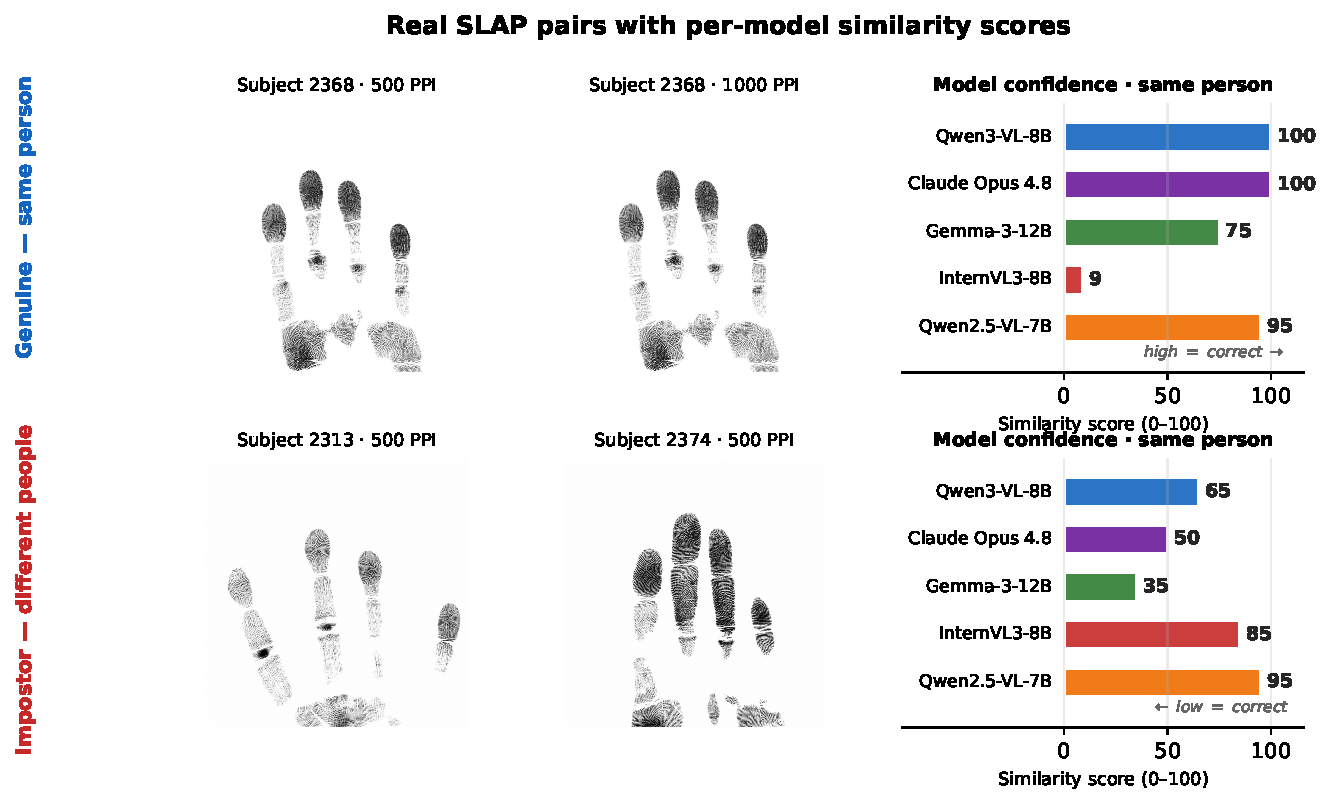
\includegraphics[width=0.96\textwidth]{fig_qualitative.pdf}
  \caption{Real SLAP pairs from SD302b with each model's
    similarity score (0--100). \textbf{Top:} a mated pair (subject~2368,
    500 vs.\ 1000~PPI). Every model but InternVL3-8B reports high
    confidence, while InternVL3 inverts and returns~9. \textbf{Bottom:} a
    non-mated pair (subjects~2313 and~2374). Qwen3-VL-8B, Claude, and Gemma
    assign lower confidence, whereas InternVL3-8B~(85, inverted) and
    Qwen2.5-VL-7B~(95, saturated) falsely accept it. Bars use the per-model
    colors of Fig.~\ref{fig:roc}, and the italic cue marks which direction
    is correct for each pair.}
  \label{fig:qualitative}
\end{figure*}

Figure~\ref{fig:roc} plots the full ROC curves for the four open-source
models and Claude Opus~4.8.
The inset shows the low-FAR operating region (FAR $\leq 0.05$),
where Qwen3-VL-8B achieves TAR~$= 100\%$ even at FAR~$= 0.1\%$.
The TAR\textsubscript{0.1\%} column of Table~\ref{tab:main_results}
reports TAR at FAR~$= 0.1\%$, the standard operational stringency target in
border biometrics. InternVL3-8B and Qwen2.5-VL-7B reach 0\% here because
their score distributions offer no threshold that holds FAR below 0.1\%
while still accepting any mated pair, a direct consequence of inverted
calibration (InternVL3) and compressed scoring (Qwen2.5).

\begin{figure}[t]
  \centering
  
\includegraphics[width=\columnwidth]{fig_roc_curves.pdf}
  \caption{ROC curves under the similarity-scoring prompt (7,832 pairs)
    for the four open-source models and the proprietary Claude Opus~4.8.
    The inset magnifies the low-FAR region (FAR $\leq 0.05$). The dotted
    vertical line marks FAR~$= 0.1\%$.
    Qwen3-VL-8B (AUC~$= 1.000$) achieves perfect discrimination, Claude
    Opus~4.8 (AUC~$= 0.953$) and Gemma-3-12B (AUC~$= 0.837$) are clearly
    functional, while InternVL3-8B and Qwen2.5-VL-7B perform near random
    (AUC~$= 0.590$ and $0.567$).}
  \label{fig:roc}
\end{figure}

\subsection{RidgeBase: Verification Under Independent Captures}
\label{sec:rb_results}

The SD302b results above leave one question open: does any model actually
match ridges, or does the single-capture pair structure let appearance
similarity stand in for identity (Section~\ref{sec:perfect})? RidgeBase answers
it directly, because its mated pairs are independent captures
(Section~\ref{sec:rb_pairs}). We report two evaluations---prompt-free embedding
matching and the similarity-scoring prompt---on the same 1{,}484-pair balanced
manifest, with results in Table~\ref{tab:ridgebase_main}.

% ── RidgeBase results table (embedding + similarity scoring) ─────────────────
\begin{table*}[t]
\centering
\caption{Verification results on RidgeBase (independent-capture, four-finger
  contactless; 592 genuine vs.\ 592 primary impostors, device-matched). We
  report prompt-free \textbf{embedding} matching (cosine on vision-encoder
  features; not available for the proprietary APIs) and the
  \textbf{similarity-scoring} prompt, using the same AUC/EER/TAR metrics as
  Table~\ref{tab:main_results}. Unlike SD302b, mated pairs here are separate
  photographs, so this table reads as the independent-capture check on the
  SD302b ranking. Numbers in red are pending the running evaluation.}
\label{tab:ridgebase_main}
\renewcommand{\arraystretch}{1.25}
\setlength{\tabcolsep}{5pt}
\footnotesize
\begin{tabular}{c l cc ccccc}
\toprule
& & \multicolumn{2}{c}{\cellcolor{grpScore}\textbf{Embedding (cosine)}}
  & \multicolumn{5}{c}{\cellcolor{grpBin}\textbf{Similarity-Scoring Prompt}} \\
\cmidrule(lr){3-4}\cmidrule(lr){5-9}
\textbf{\#} & \textbf{Model}
  & \textbf{AUC} & \textbf{EER}
  & \textbf{Gen} & \textbf{Imp} & \boldmath{$\Delta$} & \textbf{AUC} & \textbf{EER} \\
\midrule
1 & Qwen3-VL-8B     & 0.469 & 54.6\% & 68.3 & 66.1 & $+$2.2 & 0.558 & 43.6\% \\
2 & Qwen2.5-VL-7B   & 0.400 & 58.1\% & 83.3 & 81.3 & $+$2.0 & 0.550 & 44.9\% \\
3 & InternVL3-8B    & 0.434 & 56.2\% & 56.5 & 60.2 & $-$3.7 & 0.504 & 51.4\% \\
4 & Gemma-3-12B     & 0.509 & 49.3\% & 62.3 & 62.4 & $-$0.1 & 0.505 & 48.7\% \\
\midrule
5 & Claude Opus 4.8 & ---   & ---    & \ph{Gen} & \ph{Imp} & \ph{$\Delta$} & \ph{AUC} & \ph{EER} \\
6 & GPT-5.6-sol     & ---   & ---    & \ph{Gen} & \ph{Imp} & \ph{$\Delta$} & \ph{AUC} & \ph{EER} \\
\bottomrule
\end{tabular}
\end{table*}

\textbf{The perfect SD302b separation does not replicate.} On independent
captures, no open-source model separates genuine from impostor pairs above
chance. Embedding matching gives AUC between $0.400$ and $0.509$ across the
four models (Qwen2.5-VL-7B $0.400$, InternVL3-8B $0.434$, Qwen3-VL-8B $0.469$,
Gemma-3-12B $0.509$), and the similarity-scoring prompt does no better,
spanning $0.504$--$0.558$ with equal-error rates of $43.6$--$51.4\%$. The
genuine and impostor score distributions are nearly coincident: mean
similarity separations $\Delta$ range from $+2.2$ (Qwen3-VL) to $-3.7$
(InternVL3, i.e.\ inverted). Most strikingly, Qwen3-VL-8B---which reached
AUC~$= 1.000$ on SD302b---falls to $0.469$ (embedding) and $0.558$ (prompted)
here. This is the empirical counterpart to the resolution-shortcut argument of
Section~\ref{sec:perfect}: once mated pairs are no longer two views of one
image, the signal that produced a perfect SD302b score is absent
(Figure~\ref{fig:contrast}).

\begin{figure*}[t]
  \centering
  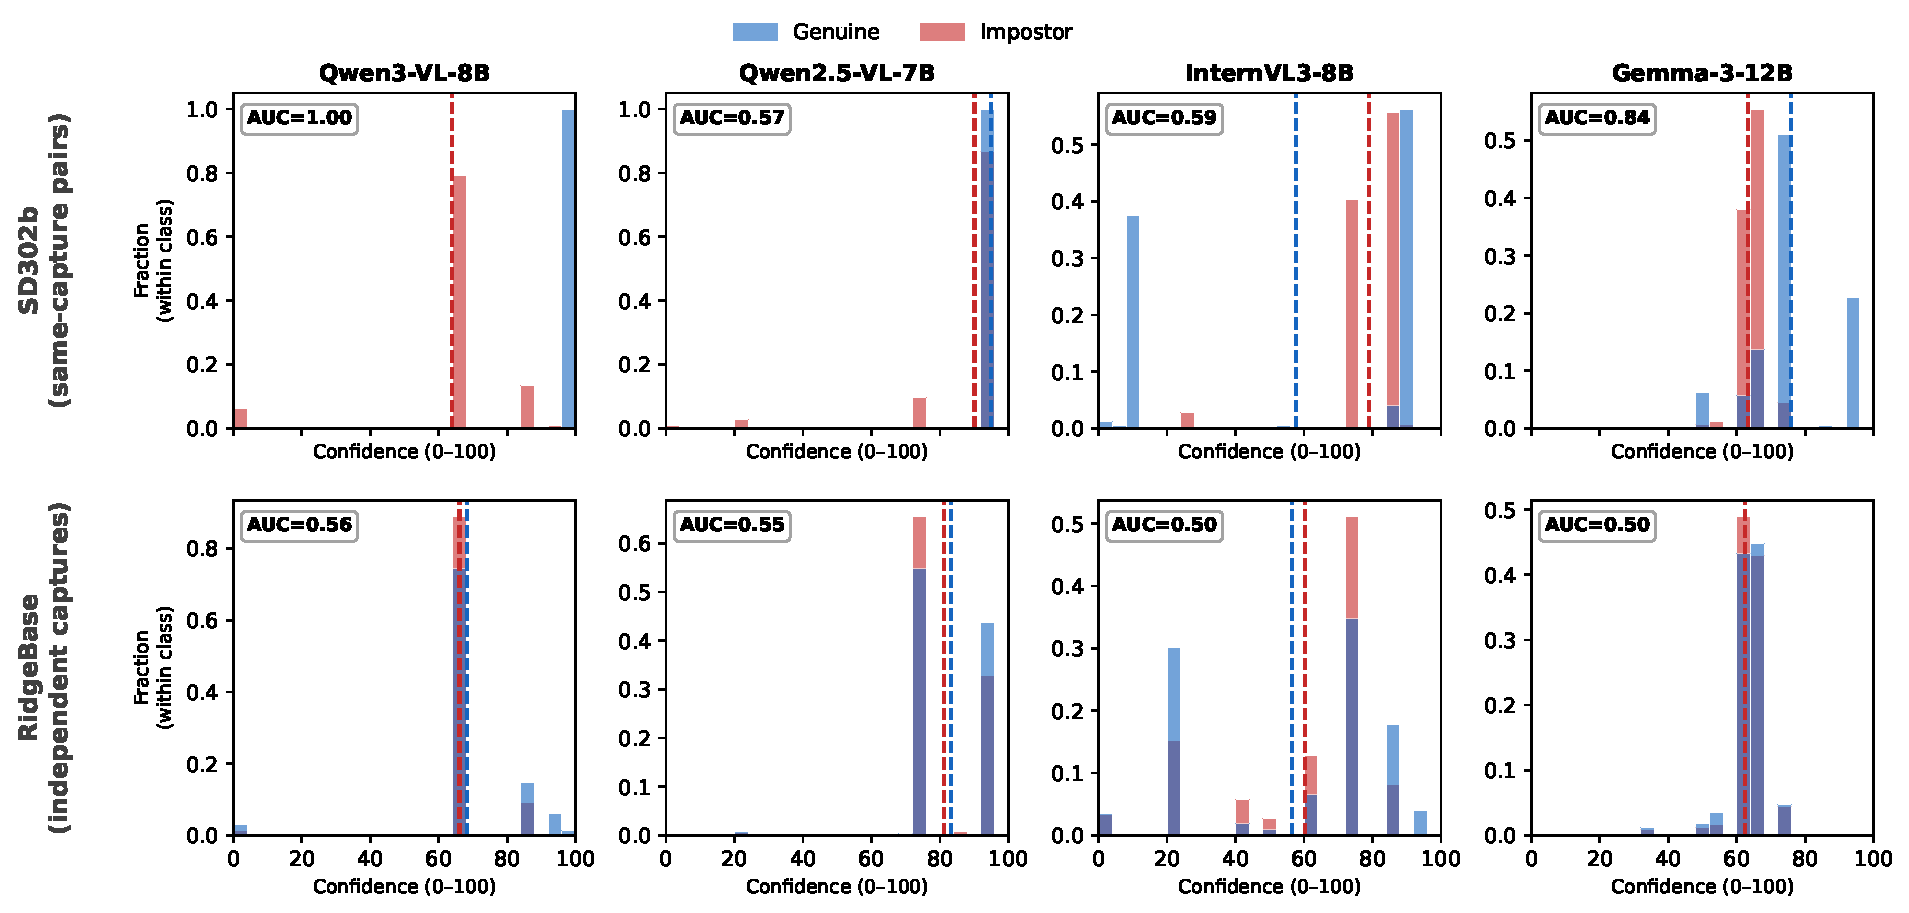
\includegraphics[width=\textwidth]{fig_sd302b_vs_ridgebase.pdf}
  \caption{\textbf{The perfect SD302b score is an artifact of pair
    construction.} Similarity-scoring distributions (within-class normalized)
    for the four open-source models. \textbf{Top:} SD302b, where each mated pair
    is the 500 and 1000~PPI rendering of one capture---genuine (blue) and
    impostor (red) separate, and Qwen3-VL-8B reaches AUC~$= 1.000$.
    \textbf{Bottom:} RidgeBase, where mated pairs are \emph{independent}
    captures---the two distributions become coincident and every model falls to
    AUC~$\approx 0.5$. The collapse from top row to bottom is the near-duplicate
    shortcut being removed.}
  \label{fig:contrast}
\end{figure*}

\begin{figure}[t]
  \centering
  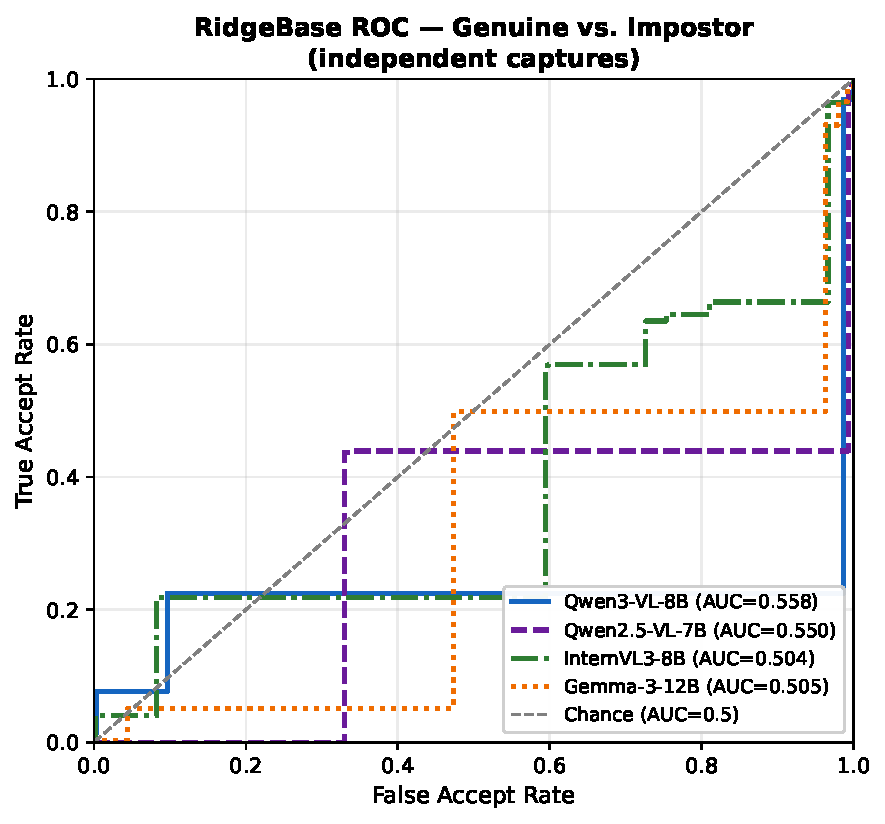
\includegraphics[width=0.82\columnwidth]{fig_ridgebase_roc.pdf}
  \caption{ROC on RidgeBase (genuine vs.\ primary impostor, independent
    captures). All four models track the chance diagonal (AUC~$0.50$--$0.56$),
    in contrast to their SD302b behavior.}
  \label{fig:rb_roc}
\end{figure}

\textbf{Cross-sensor split.} Comparing the same-device and cross-device
subsets isolates how much of any residual signal is sensor consistency rather
than identity. What little signal exists is sensor consistency: Qwen3-VL-8B,
the strongest case, scores $0.644$ on same-device genuine pairs
(Apple$\leftrightarrow$Apple or Google$\leftrightarrow$Google) but collapses to
$0.491$---exactly chance---on cross-device pairs
(Apple$\leftrightarrow$Google). Every model shows the same direction, with
same-device AUC above cross-device AUC. Because the construction holds device
composition equal between genuine and impostor sets, this gap cannot be
attributed to device makeup; it shows the models are matching capture
appearance, and lose even that when the sensor changes.

\textbf{Diagnostic impostors (same person, different hand).} These pairs share
every identity-level cue---same person, skin tone, lighting, background---but
differ in the actual fingers. Every model is at chance at separating a
subject's genuine pairs from their own opposite-hand pairs (AUC $0.523$--$0.582$
across the four models), i.e.\ it cannot tell a person's left hand from their
right. A model doing fingerprint matching would score these as confidently
non-mated; instead they are scored like genuine pairs. Together with the
embedding result and the cross-sensor collapse, this is the core mechanism
evidence that current MLLMs perform appearance matching rather than fingerprint
matching on four-finger images (Figure~\ref{fig:rb_diag}).

\begin{figure}[t]
  \centering
  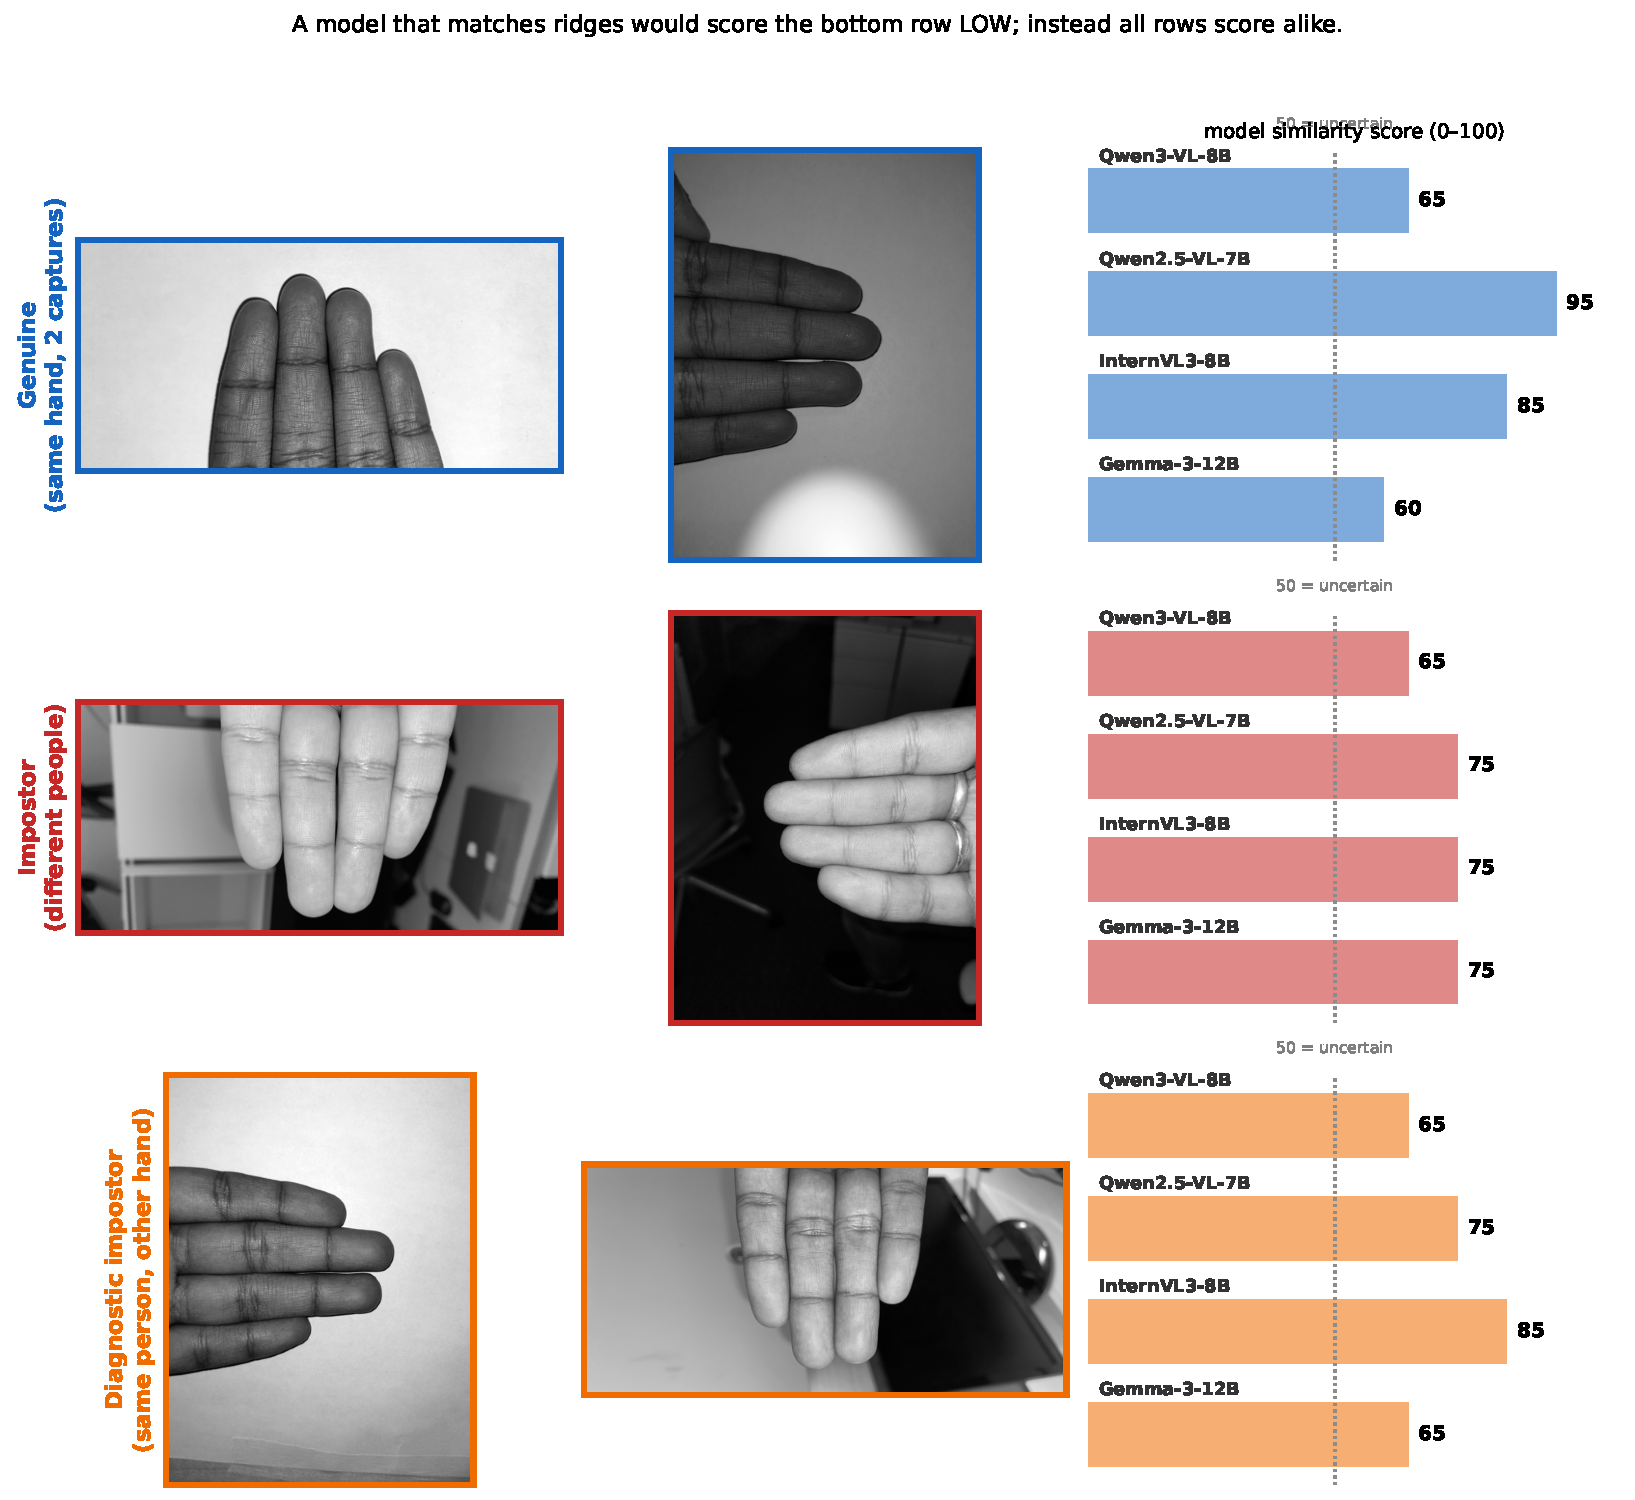
\includegraphics[width=\columnwidth]{fig_ridgebase_diagnostic.pdf}
  \caption{\textbf{Diagnostic impostors.} A real genuine pair (same hand, two
    captures), a primary impostor (different people), and a diagnostic impostor
    (\emph{same person, opposite hand}), each shown with the four models'
    similarity scores. A model comparing ridge structure would score the bottom
    row low; instead all three rows receive similar scores---e.g.\ Qwen3-VL-8B
    returns~65 for all three---showing the models cannot distinguish a person's
    two hands and are keyed on global appearance.}
  \label{fig:rb_diag}
\end{figure}

\subsection{Demographic Fairness}
\label{sec:fairness}

FaceRecBench reports that the best-performing face-verification MLLM also
exhibits the strongest demographic bias~\cite{facerecbench2025}.
We test whether the same pattern holds on SLAP fingerprints. Two scope notes
apply. This analysis uses SD302b, the only one of our two datasets with
demographic labels (RidgeBase provides none), so it necessarily characterizes
the same-capture similarity-scoring behavior of Section~\ref{sec:results}---which
Section~\ref{sec:perfect} shows is near-duplicate sensitivity rather than
verification---broken down by subgroup, not verification fairness per se. It is
best read as whether that behavior is uniform across groups; a verification
fairness audit would require an independent-capture dataset with demographics,
which we do not have.
Using the demographic metadata in our pair manifest, we recompute
similarity-scoring performance within demographic subgroups: a genuine
pair is assigned to a subgroup by its subject's attribute, and an impostor
pair is counted within a subgroup only when \emph{both} subjects share that
attribute. We restrict this analysis to the three discriminating models
(Qwen3-VL-8B, Claude Opus~4.8, Gemma-3-12B), since subgroup breakdowns of
the two near-random models are uninformative, and to subgroups with
sufficient support among the 88~clean subjects (gender; White and Black
race; three age bands). Asian, ``other,'' and ``no answer'' race groups
($\leq 6$ subjects) are excluded as too small for reliable per-group
error-rate estimates.

\begin{table}[t]
\centering
\caption{Per-subgroup similarity-scoring performance (AUC / EER\%) for the
  three discriminating models. $n_g$/$n_i$ are the genuine and within-group
  impostor pair counts. Small subgroups (Black, 18--30) are reported with
  caution. Qwen3-VL-8B is uniform at AUC~$= 1.000$ across all groups, which
  must be read alongside the perfect-score caveat of
  Section~\ref{sec:perfect}.}
\label{tab:fairness}
\renewcommand{\arraystretch}{1.2}
\setlength{\tabcolsep}{3.5pt}
\footnotesize
\begin{tabular}{l rr ccc}
\toprule
\textbf{Subgroup} & \textbf{$n_g$} & \textbf{$n_i$}
  & \textbf{Qwen3} & \textbf{Claude} & \textbf{Gemma} \\
\midrule
Male    &  70 & 1190 & 1.000 / 0.0 & 0.945 / 13.2 & 0.810 / 15.6 \\
Female  & 106 & 2756 & 1.000 / 0.0 & 0.960 / 10.5 & 0.854 / 14.8 \\
\midrule
White   & 122 & 3660 & 1.000 / 0.0 & 0.950 /  7.4 & 0.806 / 18.3 \\
Black   &  34 &  272 & 1.000 / 0.0 & 0.957 / 11.6 & 0.968 /  4.4 \\
\midrule
18--30  &  26 &  156 & 1.000 / 0.0 & 0.967 /  6.1 & 0.815 / 19.2 \\
31--45  &  76 & 1406 & 1.000 / 0.0 & 0.944 / 13.8 & 0.826 / 15.8 \\
46+     &  74 & 1332 & 1.000 / 0.0 & 0.957 / 10.6 & 0.858 / 13.5 \\
\bottomrule
\end{tabular}
\end{table}

\begin{figure*}[t]
  \centering
  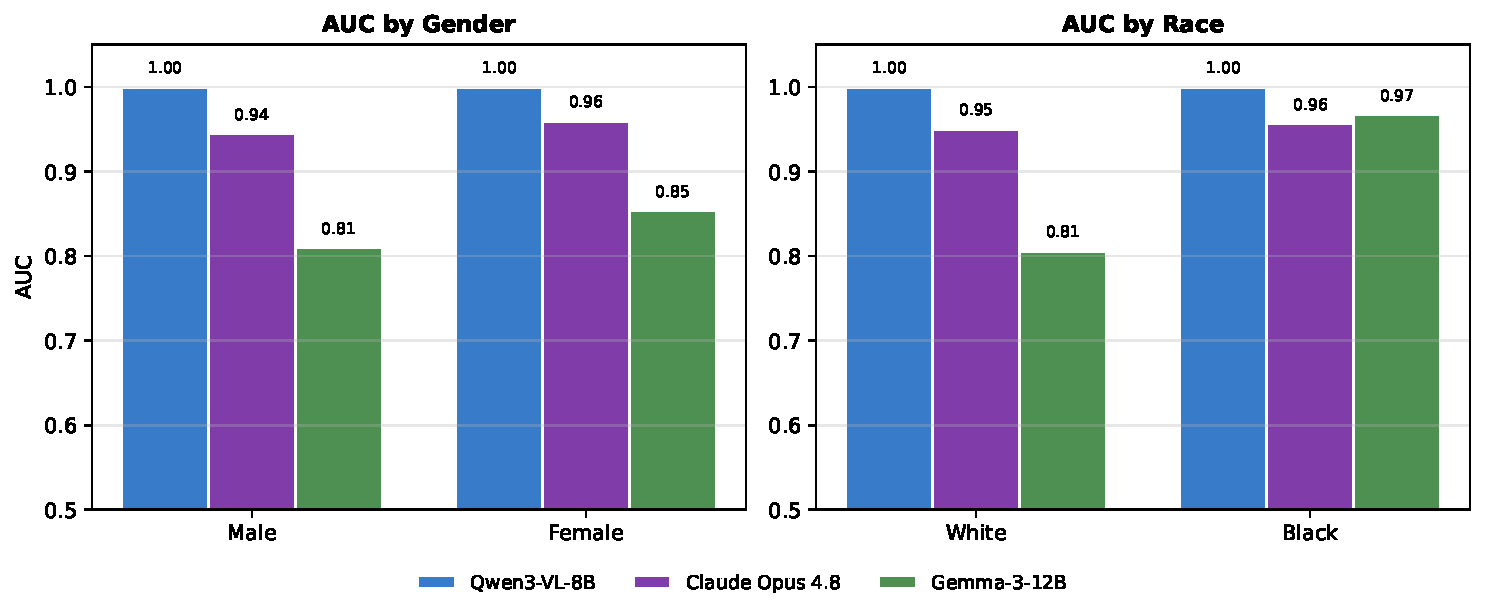
\includegraphics[width=0.92\textwidth]{fig_fairness.pdf}
  \caption{Per-subgroup AUC by gender and race for the three discriminating
    models. Qwen3-VL-8B is uniformly perfect; Claude Opus~4.8 shows small
    gaps ($\leq$1.5~AUC points by gender); Gemma-3-12B shows the largest
    disparities. The Black race group is small ($n_i = 272$), so Gemma's
    high value there is reported with caution.}
  \label{fig:fairness}
\end{figure*}

Table~\ref{tab:fairness} and Figure~\ref{fig:fairness} report the results.
The apparent pattern runs \emph{opposite} to the one FaceRecBench
describes: on SLAP data it is the stronger models that look fairer. We
offer this as a tentative observation rather than an established finding,
since the subgroup sizes are too small to support a firm conclusion.
Claude Opus~4.8 varies by at most 1.5~AUC points across gender
(male 0.945, female 0.960) and by 0.7 across the White/Black comparison.
The weakest discriminating model, Gemma-3-12B, shows the widest spread,
with a 4.4-point gender gap and an EER swing from 18.3\% to 4.4\% between
the White and Black groups. That Black subgroup rests on only 272
within-group non-mated pairs from 17 subjects, so neither its values nor
any disparity computed from them should be over-interpreted.
Qwen3-VL-8B is uniformly perfect (AUC~$= 1.000$) in every subgroup. This is
equally consistent with a group-invariant representation and with the
non-identity shortcut discussed in Section~\ref{sec:perfect}, and the
fairness data alone cannot distinguish the two.
To the extent that the data support any reading at all, demographic
disparity here tracks \emph{weakness} rather than strength: the models
carrying the least discriminative signal are also the ones that distribute
it least evenly.
Given a clean pool of 88~subjects, several small subgroups, and a single
source database, we treat these results as an initial probe that generates
hypotheses for a larger study, not as a definitive audit.

\subsection{Relationship to Prior Work}

Direct numerical comparison with FPBench~\cite{fpbench2025} is not
appropriate and we do not attempt it.
FPBench evaluates individual rolled and plain impressions from FVC
competition datasets and NIST SD302d/SD301a under a four-option
multiple-choice format; SLAPBench evaluates four-finger simultaneous
captures from NIST SD302b under a two-option binary or continuous
scoring format.
The datasets, image types, task formats, and evaluation metrics differ
at every level.
Placing numbers from both benchmarks in the same table would imply
comparability that does not exist and would mislead the reader.

What FPBench does establish, and what our results confirm, is the
qualitative pattern: binary prompting on fingerprint images produces
collapse or near-collapse in open-source models regardless of image
type, and the failure mode is consistent across both individual-finger
and SLAP formats.
SLAPBench does not set out to surpass FPBench's numbers. Its contribution
is to establish the first SLAP-specific baseline and to show that continuous
scoring prompts expose whatever discriminative signal a model has, which binary
prompting suppresses---a signal that, on genuinely independent captures, turns
out to be at chance (Section~\ref{sec:rb_results}).
These two benchmarks address different problems and should be read
as complementary, not competing.

% ────────────────────────────────────────────────────────────────────────────
\section{Discussion}
\label{sec:discussion}

\subsection{Why Binary Prompts Collapse on SLAP Data}

The collapse to ``same person'' in five of ten binary configurations is not
random failure. It follows a consistent pattern that points to a specific
mechanism.
Every collapsed run has FRR~$= 0\%$ and FAR~$\geq 96.4\%$: the model never
rejects a mated pair and accepts virtually every impostor pair.
This is the signature of a model whose prior probability for ``same
person'' is so high that no visual evidence moves it past the decision
threshold toward ``B.''

We identify two structural reasons why this prior is stronger for SLAP
images than for the individual-finger images used in FPBench.
First, any two SLAP images of a human hand share the same gross morphology:
four fingers, roughly similar spacing, similar skin texture, and similar
orientation.
The global visual similarity between any two SLAP images is far higher than
between two rolled single-finger impressions, where the absence of
surrounding fingers makes inter-subject differences more salient. This
holds whether the SLAP pair is mated or not.
Every SLAP pair therefore satisfies the surface-level similarity prior
regardless of identity, leaving the model with no visual trigger strong
enough to override it.

Second, the task-description prompt states explicitly that ``the same
person's fingers produce slightly different images each time,'' and it
increased collapse rather than reducing it.
We hypothesize that the prompt leads the model to read observed visual
differences as expected noise instead of discriminating evidence.
In language model terms, it primes a schema in which variation is a
property of mated pairs, which lowers the decision threshold for ``same''
across all inputs.
The behavior is consistent with the language component acting as a prior
over the task description, since the model encounters the phrase ``same
person'' twice before it sees either image and anchors on that framing
before processing any visual evidence.
For benchmark design, the implication is that naturalistic domain
descriptions can make collapse \emph{worse} rather than better by
legitimizing visual differences as irrelevant.

This account also explains the one exception.
Claude Opus~4.8 is the only model that resists collapse under both
prompts, and it does so in the manner the mechanism predicts: rather than
defaulting to ``same,'' it rejects roughly half of all impostor pairs even
under the task-description prompt (FAR 50.9\%) and four-fifths under
zero-shot (FAR 20.2\%).
A model able to extract identity-discriminating evidence strong enough to
overcome the surface-similarity prior is not forced into the degenerate
``same'' response; the prior biases the decision but does not determine it.
On this view, collapse is the behavior of a model whose visual evidence is
too weak to compete with its linguistic prior, not an unavoidable
consequence of the binary format itself.
The same format that collapses four open-source models leaves the
strongest model balanced, which reframes collapse as a capability
threshold rather than a fixed property of binary prompting.

\subsection{Why Similarity Scoring Breaks Collapse}

The scoring prompt resolves the same underlying problem by changing what
the model is asked to optimize.
Under binary prompting, the model must commit to a categorical label
against its own prior; the prior wins.
Under scoring, the model places a continuous estimate on a calibrated
scale, a task that requires reporting a degree of confidence rather than
crossing a decision boundary.
This framing lets the model's uncertainty about impostor pairs surface as a
lower score instead of being suppressed into the same ``A'' response it
gives to mated pairs.

The scoring prompt eliminates collapse in all four open-source models, but
the resulting distributions show that scoring is necessary without being
sufficient. It surfaces whatever discriminative signal a model has; it does
not confer any (and on SD302b that signal is near-duplicate sensitivity, not
verification).
Figure~\ref{fig:score_fail} shows the two models with the weakest signal even
under scoring, InternVL3-8B and Qwen2.5-VL-7B.

\begin{figure}[t]
  \centering
  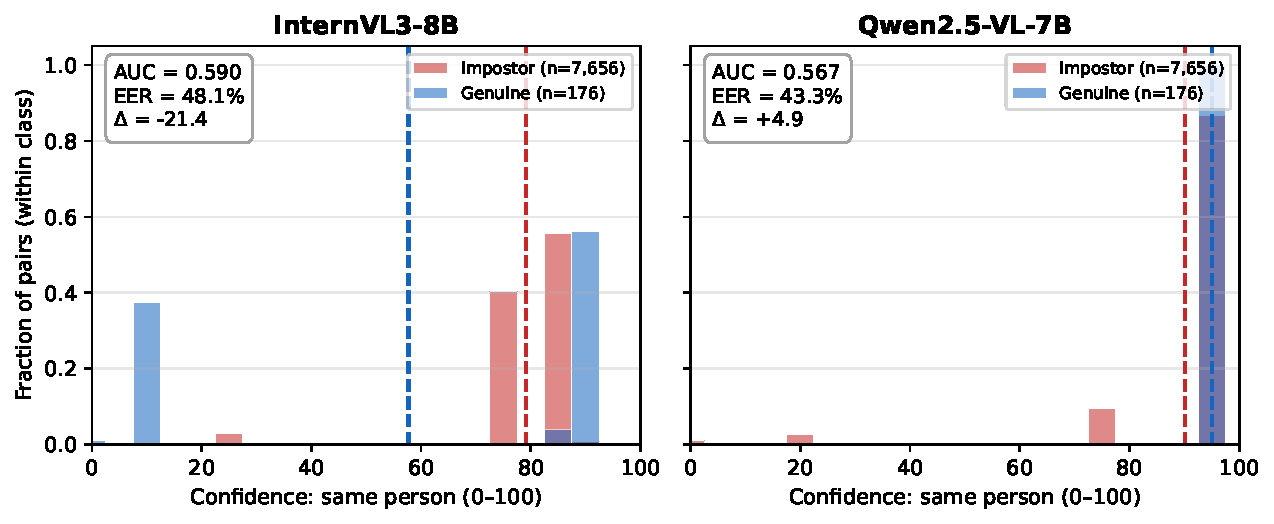
\includegraphics[width=0.86\columnwidth]{fig_score_dist_failed.pdf}
  \caption{The two models that fail under similarity scoring (7,832 pairs;
    same normalization and annotations as Fig.~\ref{fig:score_strong}).
    InternVL3-8B is \emph{inverted}: its genuine distribution is bimodal
    and its impostor mass sits \emph{above} the genuine mean
    ($\Delta = -21.4$). Qwen2.5-VL-7B is \emph{compressed}: both classes
    pile up near 95 ($\Delta = +4.9$), leaving no usable threshold. Both
    yield AUC near the 0.5 random baseline.}
  \label{fig:score_fail}
\end{figure}

\textbf{InternVL3-8B} is the most striking failure: its scores are
\emph{inverted}, assigning higher confidence to impostor pairs than to
genuine ones (Fig.~\ref{fig:score_fail}, Table~\ref{tab:main_results}).
We hypothesize that its vision encoder keys on fine-grained ridge texture,
which exhibits stronger local contrast across two different subjects than
between two captures of the same finger (which differ mainly in pressure
and scale); the scoring prompt then faithfully reports this signal, but
in the wrong direction.
Whatever the cause, scoring cannot manufacture discrimination that the
underlying representation does not encode.

\textbf{Qwen2.5-VL-7B} fails differently: its scores are ordered
correctly but compressed into a narrow high-confidence band, leaving too
little separation for reliable thresholding (Table~\ref{tab:main_results}).
This is the scoring-domain signature of the same surface-level similarity
prior that drives its binary collapse. The model is nearly certain that
every SLAP pair is a match, and the scoring format only partially relaxes
that certainty.

\textbf{Qwen3-VL-8B}, \textbf{Claude Opus~4.8}, and \textbf{Gemma-3-12B}
are the models whose scores separate the two classes
(Table~\ref{tab:main_results}), with Claude producing the widest
genuine--impostor gap of any model ($+$42.9~pts) and Qwen3 the cleanest
ranking.

Two hypotheses explain why scoring unlocks capability for the stronger
models but not the others.

\textbf{H1: Calibrated anchors direct visual attention.}
The scoring prompt instructs the model \emph{where to look}
(ridge flow, minutiae) and \emph{what to report} (a confidence value on
a calibrated scale), rather than forcing a binary commit.
The superior visual reasoning of Qwen3 and Claude may allow them to act on
these anchors, whereas InternVL3 and Qwen2.5 appear to lack the underlying
visual capability to leverage them.

\textbf{H2: Instruction-tuning on similarity scoring tasks.}
All four open-source models are trained on corpora that include aesthetic
scoring and similarity comparison tasks.
Qwen3's more recent and extensive training may provide stronger calibration
for the scoring format, an advantage that appears to diminish for the older
architectures as the task shifts from generic similarity to forensic
fingerprint discrimination.

H1 is the most actionable hypothesis: \textbf{scoring prompts with
calibrated anchors are a more effective probe of MLLM biometric
capability than binary forced choice, but only when the model
architecture has sufficient visual reasoning to exploit them.}

\subsection{A Perfect Score Is a Diagnostic, Not a Capability Claim}
\label{sec:perfect}

Qwen3-VL-8B attains AUC~$= 1.000$ with EER~$= 0.0\%$. We do not present
this as a capability result, and we argue that it should not be read as
one. Our position is that the number is explained by the structure of the
protocol rather than by the model's verification ability, and this
subsection sets out the evidence for that conclusion. We treat the episode
as the most useful finding in the paper for benchmark designers, because it
shows how readily a SLAP verification protocol can manufacture a perfect
score.

The behavior underlying the number is narrow and revealing. Qwen3-VL-8B
assigns a score of \emph{exactly} 100 to all 176 mated pairs: the mated
score distribution has a single distinct value. Its non-mated scores, by
contrast, take only seven distinct values
($\{0, 30, 45, 65, 85, 90, 95\}$, mean 63.8), and \emph{no} non-mated pair
is ever scored above 95. Perfect separation is therefore not the product of
a finely graded similarity judgment. It follows from a coarsely quantized
output in which one response, 100, is emitted for every cross-resolution
pair and never for any same-resolution pair. Any mechanism that saturates
the mated class in this way reproduces AUC~$= 1.000$ exactly, whether or not
it involves comparing ridge structure, and a model performing genuine
forensic comparison would be expected to express at least some graded
uncertainty across 176 distinct subjects.

The \textbf{resolution shortcut} is the explanation that fits this signature
most economically. As Section~\ref{sec:pairs} notes, SD302b supplies one
SLAP capture per subject and finger position, so mated pairs must be built
across resolutions (1000~PPI vs.\ 500~PPI) while non-mated pairs are
same-resolution (500~PPI vs.\ 500~PPI). A model that merely detects whether
two images differ in resolution or in the appearance statistics that
downsampling leaves behind can therefore separate the classes perfectly
without performing identity comparison at all. Such a detector would
saturate the mated class exactly as observed. This mechanism is sufficient
on its own to produce the result, it requires no verification capability
whatsoever, and it is the reading we regard as most likely.

A related and partly deflationary reading is \textbf{near-duplicate
detection}. Because mated pairs are two renderings of one capture, they are
near-duplicates at the signal level, and low-level ridge correspondence
between them is far stronger than anything a deployed matcher encounters
when comparing two independent impressions. Detecting that correspondence
would also drive confidence to the ceiling without implying border-grade
verification.

\textbf{Memorization} is the reading we can most confidently set aside.
SD302b is a public NIST release, so contamination of Qwen3's pretraining
corpus cannot be excluded outright, but the evidence runs against it. Had
the model memorized SD302b identity labels, that knowledge should transfer
across prompts; instead its zero-shot binary FAR is 26.5\% and it collapses
entirely under task description, which is inconsistent with rote recall.
Memorization also fails to explain why no other model reproduces the
result. Claude Opus~4.8, the strongest system we tested, reaches
AUC~$= 0.953$ with mated confidence averaging 91.3 rather than pinned
at 100. That a frontier model stops short of perfect separation makes
Qwen3's exact-100 behavior look less like superior recall and more like a
different mechanism operating altogether.

The remaining reading, \textbf{genuine cross-resolution discrimination}---under
which Qwen3 recognizes shared ridge structure across the two renderings and
reports maximal confidence for sound reasons---is the one a capability claim
would require. We regarded it as the least likely of the four even before
testing, since it must explain why a capability strong enough to be flawless
here leaves the same model collapsing to 98.9\% FAR under a binary prompt on
the same images.

\textbf{The RidgeBase evaluation settles it.} Rather than only specifying the
control, we ran it: RidgeBase supplies genuinely independent captures of each
hand (Section~\ref{sec:rb_results}), which removes the resolution and
near-duplicate cues at their source. On those pairs Qwen3-VL-8B falls to
AUC~$= 0.469$ (embedding) and $0.558$ (scoring)---chance---and every other
model does the same. A model with genuine cross-resolution verification
ability would have carried at least part of that skill to independent
captures; none did. This excludes the genuine-discrimination reading and
confirms that the perfect SD302b score was driven by the mated-pair
construction, not by identity comparison. (A matched-resolution SD302b control,
in which non-mated pairs are also formed 1000~PPI vs.\ 500~PPI, remains a
valid within-dataset check and is consistent with this conclusion.)

The honest summary is therefore firm rather than tentative. Qwen3-VL-8B
separates SD302b's mated and non-mated pairs perfectly under scoring; that
separation is near-duplicate detection, not identity comparison, as the
collapse to chance on independent RidgeBase captures demonstrates; and no
operational verification capability should be inferred from it. The broader
lesson generalizes past this benchmark: when a dataset offers only one capture
per subject, the mated class must be constructed by some transformation of that
capture, and any such transformation risks becoming the very cue the model
learns to read. Near-perfect results on MLLM biometric benchmarks warrant a
protocol audit---or, better, an independent-capture dataset---before they
warrant belief.

\subsection{The Left-Hand / Right-Hand Asymmetry}

Under zero-shot prompting, a moderate hand asymmetry appears in
Qwen3-VL-8B, whose FAR is 24.0\% on FRGP~14 (left hand) against 29.0\% on
FRGP~13 (right hand), a 5.0-point gap favoring the left.
InternVL3-8B, Qwen2.5-VL-7B, and Gemma-3-12B are near-symmetric across the
two positions, with FAR gaps of 1.1, 3.6, and 2.7 points respectively.
Claude Opus~4.8 shows a comparable 4.7-point gap in the \emph{opposite}
direction, favoring the right hand (FRGP~13 FAR 17.8\% versus FRGP~14
22.5\%), so the two strongest models disagree about which hand is easier.
Both FRGPs contain identical pair counts drawn from the same 88 subjects,
which rules out dataset composition as a cause. The disagreement between
models points instead to model-specific pretraining priors rather than to
any universal property of SLAP images.

One candidate prior is the relative frequency of each hand in
pretraining data: a model that has seen fewer left-hand images may rely
more on ridge-level features than on global hand morphology, shifting its
per-hand error rates. Because the direction differs across models, this
prior must be model-specific; distinguishing it from dataset-specific
effects requires evaluation on a second dataset and is deferred to future
work.

\subsection{Limitations}
\label{sec:limitations}

Three limitations bound what the present results establish, and we state
them alongside the findings each one does and does not touch.

\textbf{Mated-pair construction.}
SD302b provides a single SLAP capture per subject and finger position, so a
mated pair can only be formed across the two resolutions of that one
capture (Section~\ref{sec:dataset}). Mated pairs are consequently
cross-resolution while non-mated pairs are same-resolution, and a model can
in principle exploit that asymmetry instead of comparing ridge structure.
This bears squarely on the top of the ranking, and it is why we decline to
read Qwen3-VL-8B's AUC~$= 1.000$ as evidence of verification capability
(Section~\ref{sec:perfect}). It does not, however, bear on the paper's
central findings. Positive-bias collapse is measured by the rate at which a
model accepts non-mated pairs, which are same-resolution by construction
and involve no cross-resolution comparison at all; the collapse of four
open-source models under task-description prompting, Gemma-3-12B's collapse
under zero-shot, Claude Opus~4.8's resistance to both, and the removal of
collapse by similarity scoring are all unaffected. A matched-resolution
non-mated set is the control that would extend the same confidence to the
capability ranking on SD302b. Beyond that within-SD302b control, the RidgeBase
evaluation (Section~\ref{sec:rb_results}) addresses the confound at its root:
its mated pairs are independent captures, so the perfect SD302b separation can
be tested rather than only caveated, and the RidgeBase result confirms the
shortcut interpretation: on independent captures every model collapses to
chance (Section~\ref{sec:rb_results}), so the near-perfect SD302b scores
reflected near-duplicate detection, not verification capability.

\textbf{Model coverage.}
Our proprietary coverage is a single system. FPBench reports that Gemini
2.5 Pro leads open-source models by roughly 4 percentage points on
single-finger tasks~\cite{fpbench2025}, and whether the collapse resistance
we observe in Claude Opus~4.8 is a property of frontier-scale models
generally or specific to Claude cannot be settled with one data point.

\textbf{Scale of the fairness analysis.}
The clean pool is 88~subjects, the Black and 18--30 subgroups are small,
and the Asian and ``other'' groups are too small to evaluate. We report
Section~\ref{sec:fairness} as an initial probe on a single database, and
the inverted disparity pattern it suggests should be treated as a
hypothesis for a larger and more balanced study rather than as an audit.

Finally, we note that SLAPBench compares MLLMs against one another and not
against a deployed fingerprint system. Anchoring the similarity scores to a
commercial matcher such as VeriFinger~\cite{verifinger} at its standard
operating threshold would place these models on an absolute,
deployment-referenced scale; we set this out as future work rather than a
claim of the present study.

\subsection{Future Work}

Six directions follow directly from these findings.
(i)~\textbf{Matched-resolution controls}: the most immediate priority is
to rebuild the non-mated pairs as 1000~PPI vs.\ 500~PPI comparisons so
that both classes share the same resolution structure. This removes the
asymmetry described in Section~\ref{sec:pairs} and tests whether the
strongest results, above all Qwen3-VL-8B's perfect separation, survive once
resolution no longer signals class.
Reporting both orderings (1000-vs-500 and 500-vs-1000) as an ablation
would further isolate any residual appearance cue.
(ii)~\textbf{Broader proprietary model evaluation}: Claude Opus~4.8 resists
binary collapse under both prompts and ranks second under scoring
(AUC~$= 0.953$, EER~$= 11.8\%$), which shows that collapse resistance
extends to at least one frontier proprietary model. Extending the
comparison to additional proprietary systems such as the OpenAI GPT-series
and Google Gemini would establish whether this robustness is general to
frontier-scale models or specific to Claude.
(iii)~\textbf{Domain-adaptive fine-tuning}: FPBench demonstrates
7--39\% improvement from jointly fine-tuning vision and language
encoders on single-finger tasks~\cite{fpbench2025}; applying the
same protocol to SLAP images would test whether the discriminative
signal present under scoring prompts can be made reliably accessible
under binary prompting after adaptation.
(iv)~\textbf{Larger-scale fairness evaluation}: extending the
demographic analysis of Section~\ref{sec:fairness} to a balanced,
multi-database subject pool that supports reliable estimates for the
small subgroups (Asian, ``other,'' youngest band) omitted here.
(v)~\textbf{Algorithmic-baseline calibration}: anchoring the MLLM
similarity scores against a traditional matcher (e.g., VeriFinger SDK
scores at the standard match threshold) would quantify how far each
model's discrimination sits from a deployed-system reference and provide
a common axis for cross-model comparison.
(vi)~\textbf{Benchmark extension}: the full SLAPBench specification
includes seven additional tasks beyond verification, namely finger count
estimation, hand laterality classification, finger localization, finger
position identification, image quality scoring, rotation estimation, and
segmentation challenge identification. Together these cover the complete
SLAP analysis pipeline. Quality-stratified (NFIQ~2) and demographic
breakdowns, along with LoRA fine-tuning of the strongest open-source
models, form part of the same extension.
These tasks are deferred to subsequent work.

% ────────────────────────────────────────────────────────────────────────────
\section{Conclusion}
\label{sec:conclusion}

We introduced SLAPBench, the first benchmark for evaluating multimodal
large language models on four-finger SLAP fingerprint verification, and
evaluated it across two datasets: NIST SD302b (contact livescan) and
RidgeBase (independent-capture contactless).
Task-description prompting collapses all four open-source models to
near-100\% FAR on \emph{both} datasets, and Gemma-3-12B collapses under
zero-shot as well, while on SD302b the proprietary Claude Opus~4.8 resists
collapse under both prompts. Collapse is thus an artifact of the prompt
format that recurs regardless of dataset.
Similarity scoring removes the collapse, but the score separation it reveals
must be read carefully. On SD302b every mated pair is the 500 and 1000~PPI
versions of one capture, so the separation---and Qwen3-VL-8B's perfect
AUC~$= 1.000$---reflects near-duplicate sensitivity, not verification. The
RidgeBase evaluation confirms this directly: given genuinely independent
captures, every model falls to chance (embedding AUC~$0.40$--$0.51$,
similarity-scoring AUC~$0.50$--$0.56$), none can separate a subject's own two
hands, and the little residual signal that exists is sensor consistency rather
than identity. No current MLLM we tested performs four-finger fingerprint
verification; they match global appearance.
The most transferable lesson concerns benchmark construction. Whenever a
biometric dataset offers only one capture per subject, the mated class must be
synthesized from that capture, and the synthesis itself can become the cue a
model learns to read; near-perfect MLLM results in such a setting call for a
protocol audit, or an independent-capture dataset, before they call for belief.
Immediate next steps are to complete the two proprietary systems (Claude
Opus~4.8 and a current GPT model) on RidgeBase, to anchor the scores against a
traditional matcher such as VeriFinger~\cite{verifinger}, and to test whether
domain-adaptive fine-tuning closes the gap, consistent with the gains FPBench
reports on single-finger tasks~\cite{fpbench2025}.

% ────────────────────────────────────────────────────────────────────────────
{\footnotesize
\bibliographystyle{IEEEtran}
\bibliography{references}
}

\end{document}